% ============================================================
% CARBON FIBER LAMINA MANUFACTURING & TENSILE CHARACTERIZATION
% TWO-PAGE PORTFOLIO CASE STUDY
% 01 Composites / Project 05
%
% IMPORTANT:
% 1. This file must NOT contain \documentclass, \begin{document},
%    or \end{document}.
% 2. In main.tex, place \input{coupon_testing} before \end{document}.
% 3. This script assumes the main portfolio preamble already defines:
%       DeepGreen, PolyGold, SoftGold, SoftGreen,
%       RuleGray, Muted, Ink
%    and loads tikz, graphicx, hyperref, and fontawesome5.
% 4. Upload these files to Overleaf with the exact same names:
%       Lamina Layering.png
%       Lamina Layer Rolling.JPG
%       Vacuum Bagging Panels.png
%       Autoclave.png
%       Cutting Coupon Samples.png
%       Catastrophic Laminate Failure.JPG
%       Stress Strain Plot.png
%       Q bar.png
%       S bar.png
% ============================================================

\providecommand{\CouponFailureVideo}
{https://drive.google.com/file/d/1EytOiadSSdiBPm855tiwnkO2kXlO5trU/view?usp=drive_link}

\providecommand{\CouponReportOne}
{https://drive.google.com/file/d/1XtEZSRZMTFmzKIk3v_zTwT6gxZyLEyW5/view?usp=sharing}

\providecommand{\CouponReportTwo}
{https://drive.google.com/file/d/1dq82_FQC8oGFbILCtTh4ZzD-SmT6Ute4/view?usp=drive_link}

\providecommand{\CouponReportThree}
{https://drive.google.com/file/d/1Gu54UFZfrPYRrOnVh5Dqf-ldtvUttEf5/view?usp=drive_link}

% ============================================================
% PAGE 1 — MANUFACTURING
% ============================================================

\clearpage
\thispagestyle{empty}
\hypertarget{coupon-testing}{}
\null

\begin{tikzpicture}[remember picture,overlay]

% PAGE BACKGROUND AND BARS
\fill[white] (current page.south west) rectangle (current page.north east);
\fill[DeepGreen] (current page.north west) rectangle ($(current page.north east)+(0,-0.095in)$);
\fill[PolyGold] ($(current page.north west)+(0,-0.095in)$) rectangle ($(current page.north east)+(0,-0.14in)$);
\fill[DeepGreen] (current page.south west) rectangle ($(current page.south east)+(0,0.36in)$);
\fill[PolyGold] ($(current page.south west)+(0,0.36in)$) rectangle ($(current page.south east)+(0,0.405in)$);

% HEADER
\node[anchor=north west,text=PolyGold,font=\sffamily\bfseries\fontsize{8.1}{8.7}\selectfont]
at ($(current page.north west)+(0.42in,-0.39in)$)
{01 COMPOSITES \hspace{5pt}/\hspace{5pt} PROJECT 05};

\node[anchor=north west,text=DeepGreen,font=\bfseries\fontsize{17.6}{18.7}\selectfont]
at ($(current page.north west)+(0.40in,-0.67in)$)
{CARBON FIBER COUPON MANUFACTURING \& TENSILE TESTING};

\node[anchor=north west,text=Muted,font=\sffamily\fontsize{8.15}{8.9}\selectfont]
at ($(current page.north west)+(0.42in,-1.12in)$)
{Cal Poly Composites Laboratory \hspace{7pt}\textbullet\hspace{7pt}
Team Project \hspace{7pt}\textbullet\hspace{7pt}
Summer 2025 \hspace{7pt}\textbullet\hspace{7pt}
San Luis Obispo, California};

\fill[PolyGold]
    ($(current page.north west)+(0.42in,-1.36in)$)
    rectangle
    ($(current page.north west)+(6.10in,-1.315in)$);


% OVERVIEW — LEFT COLUMN
\fill[SoftGold,rounded corners=5pt]
($(current page.north west)+(0.42in,-1.58in)$) rectangle ($(current page.north west)+(3.18in,-6.22in)$);
\fill[PolyGold]
($(current page.north west)+(0.42in,-1.58in)$) rectangle ($(current page.north west)+(0.52in,-6.22in)$);

\node[anchor=north west,text=DeepGreen,font=\sffamily\bfseries\fontsize{8.0}{8.7}\selectfont]
at ($(current page.north west)+(0.72in,-1.77in)$){PROJECT OVERVIEW};

\node[anchor=north west,align=left,text width=2.15in,text=Ink,font=\fontsize{6.18}{7.16}\selectfont]
at ($(current page.north west)+(0.72in,-2.04in)$)
{A sequence of carbon/epoxy coupon studies connected laminate manufacturing, tensile testing, and composite-property calculations. Unidirectional prepreg was cut at 0°, 90°, and $\pm45^\circ$, assembled into symmetric laminates, vacuum bagged, and cured using both out-of-autoclave and autoclave processes.\\[5pt]
The work emphasized fiber alignment, ply consolidation, specimen preparation, repeat testing, and the limits of relying on simplified theory to predict real manufactured behavior.};

\node[
    anchor=north west,
    text=DeepGreen,
    font=\sffamily\bfseries\fontsize{7.2}{7.9}\selectfont
]
at ($(current page.north west)+(0.72in,-4.22in)$)
{MY ROLE};

\node[
    anchor=north west,
    align=left,
    text width=2.12in,
    text=Ink,
    font=\fontsize{5.95}{6.85}\selectfont
]
at ($(current page.north west)+(0.72in,-4.48in)$)
{
\textbf{Team Leader.} Coordinated task delegation, project progress, and testing activities.\\[4pt]
\textbf{Manufacturing Lead.} Directed laminate layup, vacuum bagging, curing, coupon preparation, and manufacturing quality control.
};

\node[
    anchor=north west,
    text=DeepGreen,
    font=\sffamily\bfseries\fontsize{7.0}{7.7}\selectfont
]
at ($(current page.north west)+(0.72in,-5.42in)$)
{PROCESS SEQUENCE};

\node[
    anchor=north west,
    align=left,
    text width=2.12in,
    text=Ink,
    font=\fontsize{5.62}{6.38}\selectfont
]
at ($(current page.north west)+(0.72in,-5.66in)$)
{
Orient and cut plies \textbullet\ Compact layers \textbullet\ Vacuum bag and leak-check \textbullet\ Cure \textbullet\ Cut and finish coupons
};

\node[
    anchor=south west,
    text=PolyGold,
    font=\sffamily\bfseries\fontsize{6.2}{6.85}\selectfont
]
at ($(current page.north west)+(0.72in,-6.04in)$)
{0° \hspace{6pt}\textbullet\hspace{6pt} 90° \hspace{6pt}\textbullet\hspace{6pt} $\pm45^\circ$ \hspace{6pt}\textbullet\hspace{6pt} CROSS-PLY};

% IMAGE GRID — PROCESS ORDER: LAYERING, ROLLING, VACUUM BAGGING,
% AUTOCLAVE CURING, COUPON CUTTING, FINISHED COUPONS

% Top 1: Layering
\node[anchor=north west,inner sep=2.3pt,draw=DeepGreen,line width=0.65pt,rounded corners=4pt]
at ($(current page.north west)+(3.46in,-1.58in)$)
{\includegraphics[width=2.27in,height=2.15in,keepaspectratio]{\detokenize{Lamina Layering.png}}};
\node[anchor=north,align=center,inner sep=0pt,text width=2.18in,text=Muted,font=\sffamily\fontsize{5.8}{6.45}\selectfont]
at ($(current page.north west)+(4.595in,-3.84in)$)
{Ply orientation and stacking};

% Top 2: Rolling
\node[anchor=north west,inner sep=2.3pt,draw=DeepGreen,line width=0.65pt,rounded corners=4pt]
at ($(current page.north west)+(5.93in,-1.58in)$)
{\includegraphics[width=2.27in,height=2.15in,keepaspectratio]{\detokenize{Lamina Layer Rolling.JPG}}};
\node[anchor=north,align=center,inner sep=0pt,text width=2.18in,text=Muted,font=\sffamily\fontsize{5.8}{6.45}\selectfont]
at ($(current page.north west)+(7.065in,-3.84in)$)
{Ply compaction rolling};

% Top 3: Vacuum bagging
\node[anchor=north west,inner sep=2.3pt,draw=DeepGreen,line width=0.65pt,rounded corners=4pt]
at ($(current page.north west)+(8.40in,-1.58in)$)
{\includegraphics[width=2.62in,height=2.15in,keepaspectratio]{\detokenize{Vacuum Bagging Panels.png}}};
\node[anchor=north,align=center,inner sep=0pt,text width=2.48in,text=Muted,font=\sffamily\fontsize{5.8}{6.45}\selectfont]
at ($(current page.north west)+(9.71in,-3.84in)$)
{Sealed vacuum-bag assembly};

% Bottom 1: Autoclave
\node[anchor=north west,inner sep=2.3pt,draw=RuleGray,line width=0.55pt,rounded corners=4pt]
at ($(current page.north west)+(3.46in,-4.18in)$)
{\includegraphics[width=2.27in,height=1.72in,keepaspectratio]{\detokenize{Autoclave.png}}};
\node[anchor=north,align=center,inner sep=0pt,text width=2.18in,text=Muted,font=\sffamily\fontsize{5.8}{6.45}\selectfont]
at ($(current page.north west)+(4.595in,-5.98in)$)
{Autoclave cure cycle};

% Bottom 2: Coupon cutting
\node[anchor=north west,inner sep=2.3pt,draw=RuleGray,line width=0.55pt,rounded corners=4pt]
at ($(current page.north west)+(5.93in,-4.18in)$)
{\includegraphics[width=2.27in,height=1.72in,keepaspectratio]{\detokenize{Cutting Coupon Samples.png}}};
\node[anchor=north,align=center,inner sep=0pt,text width=2.18in,text=Muted,font=\sffamily\fontsize{5.8}{6.45}\selectfont]
at ($(current page.north west)+(7.065in,-5.98in)$)
{Coupon cutting and finishing};

% Bottom 3: Finished coupons
\node[anchor=north west,inner sep=2.3pt,draw=RuleGray,line width=0.55pt,rounded corners=4pt]
at ($(current page.north west)+(8.40in,-4.18in)$)
{\includegraphics[width=2.62in,height=1.72in,keepaspectratio]{\detokenize{Coupons.JPG}}};
\node[anchor=north,align=center,inner sep=0pt,text width=2.48in,text=Muted,font=\sffamily\fontsize{5.8}{6.45}\selectfont]
at ($(current page.north west)+(9.71in,-5.98in)$)
{Finished laminate coupons};

% BOTTOM TEXT PANELS
\fill[SoftGreen,rounded corners=5pt]
($(current page.north west)+(0.42in,-6.43in)$) rectangle ($(current page.north west)+(5.36in,-7.20in)$);
\draw[RuleGray,line width=0.55pt,rounded corners=5pt]
($(current page.north west)+(0.42in,-6.43in)$) rectangle ($(current page.north west)+(5.36in,-7.20in)$);
\node[anchor=north west,text=DeepGreen,font=\sffamily\bfseries\fontsize{7.55}{8.25}\selectfont]
at ($(current page.north west)+(0.66in,-6.56in)$){MANUFACTURING WORKFLOW};
\node[anchor=north west,align=left,text width=4.47in,text=Ink,font=\fontsize{5.92}{6.84}\selectfont]
at ($(current page.north west)+(0.66in,-6.80in)$)
{Prepreg was thawed, oriented, cut, layered, compacted, vacuum bagged, leak checked, thermally cured, demolded, and cut into test coupons. Manufacturing quality directly influenced the later property calculations and failure interpretation.};

\fill[SoftGold,rounded corners=5pt]
($(current page.north west)+(5.58in,-6.43in)$) rectangle ($(current page.north east)+(-0.42in,-7.20in)$);
\fill[PolyGold]
($(current page.north west)+(5.58in,-6.43in)$) rectangle ($(current page.north west)+(5.68in,-7.20in)$);
\node[anchor=north west,text=DeepGreen,font=\sffamily\bfseries\fontsize{7.55}{8.25}\selectfont]
at ($(current page.north west)+(5.88in,-6.56in)$){WHY THE PROCESS MATTERED};
\node[anchor=north west,align=left,text width=4.61in,text=Ink,font=\fontsize{5.90}{6.82}\selectfont]
at ($(current page.north west)+(5.88in,-6.80in)$)
{Coupon data are only as trustworthy as the specimens being tested. Fiber misalignment, trapped air, thickness variation, rough cutting, and grip damage can distort measured stiffness and strength.};

% FOOTER
\node[anchor=south west,text=white,font=\sffamily\bfseries\fontsize{7.1}{7.7}\selectfont]
at ($(current page.south west)+(0.42in,0.17in)$)
{\hyperlink{fuselage}{\faArrowLeft\ FIBERGLASS FUSELAGE}};
\node[anchor=south,text=white,font=\sffamily\fontsize{7.0}{7.6}\selectfont]
at ($(current page.south)+(0,0.17in)$)
{CARBON FIBER COUPONS \hspace{6pt} 1 / 2};
\node[anchor=south east,text=white,font=\sffamily\bfseries\fontsize{7.1}{7.7}\selectfont]
at ($(current page.south east)+(-0.42in,0.17in)$)
{RESULTS \& ANALYSIS \faArrowRight};

\end{tikzpicture}

% ============================================================
% PAGE 2 — TESTING, PROPERTY CALCULATION, AND FAILURE ANALYSIS
% ============================================================

\clearpage
\thispagestyle{empty}
\null

\begin{tikzpicture}[remember picture,overlay]

% PAGE BACKGROUND AND BARS
\fill[white] (current page.south west) rectangle (current page.north east);

\fill[DeepGreen]
    (current page.north west)
    rectangle
    ($(current page.north east)+(0,-0.095in)$);

\fill[PolyGold]
    ($(current page.north west)+(0,-0.095in)$)
    rectangle
    ($(current page.north east)+(0,-0.14in)$);

\fill[DeepGreen]
    (current page.south west)
    rectangle
    ($(current page.south east)+(0,0.36in)$);

\fill[PolyGold]
    ($(current page.south west)+(0,0.36in)$)
    rectangle
    ($(current page.south east)+(0,0.405in)$);

% HEADER
\node[
    anchor=north west,
    text=PolyGold,
    font=\sffamily\bfseries\fontsize{8.1}{8.7}\selectfont
]
at ($(current page.north west)+(0.42in,-0.39in)$)
{CARBON FIBER COUPONS \hspace{5pt}/\hspace{5pt} RESULTS AND ANALYSIS};

\node[
    anchor=north west,
    text=DeepGreen,
    font=\bfseries\fontsize{20.7}{21.7}\selectfont
]
at ($(current page.north west)+(0.40in,-0.67in)$)
{FROM TENSILE DATA TO LAMINA PROPERTIES};

\node[
    anchor=north west,
    text=Muted,
    font=\sffamily\fontsize{8.1}{8.8}\selectfont
]
at ($(current page.north west)+(0.42in,-1.12in)$)
{Mechanical testing, stiffness extraction, failure interpretation, and limits of theoretical prediction};

\fill[PolyGold]
    ($(current page.north west)+(0.42in,-1.36in)$)
    rectangle
    ($(current page.north west)+(5.20in,-1.315in)$);


% TOP LEFT — FAILURE PHOTO
\node[
    anchor=north west,
    inner sep=2.6pt,
    draw=DeepGreen,
    line width=0.68pt,
    rounded corners=5pt
]
at ($(current page.north west)+(3.96in,-1.58in)$)
{
    \includegraphics[
        width=3.60in,
        height=2.47in,
        keepaspectratio
    ]{\detokenize{Catastrophic Laminate Failure.JPG}}
};

\node[
    anchor=north,
    align=center,
    inner sep=0pt,
    text width=3.45in,
    text=Muted,
    font=\sffamily\fontsize{6.25}{6.95}\selectfont
]
at ($(current page.north west)+(5.76in,-4.14in)$)
{Catastrophic coupon failure after tensile loading};

% TOP CENTER/RIGHT — STRESS STRAIN
\node[
    anchor=north west,
    inner sep=2.6pt,
    draw=DeepGreen,
    line width=0.68pt,
    rounded corners=5pt
]
at ($(current page.north west)+(6.95in,-1.58in)$)
{
    \includegraphics[
        width=6.74in,
        height=2.47in,
        keepaspectratio
    ]{\detokenize{Stress Strain Plot.png}}
};

\node[
    anchor=north,
    align=center,
    inner sep=0pt,
    text width=6.56in,
    text=Muted,
    font=\sffamily\fontsize{6.25}{6.95}\selectfont
]
at ($(current page.north west)+(8.87in,-4.14in)$)
{Stress-strain regression used to estimate elastic modulus};

% TOP LEFT — PROPERTY EXTRACTION
% Top edge aligned with the catastrophic-failure image and bottom edge
% aligned with the Q-bar plot.
\fill[SoftGold,rounded corners=5pt]
    ($(current page.north west)+(0.42in,-1.58in)$)
    rectangle
    ($(current page.north west)+(3.72in,-6.20in)$);

\fill[PolyGold]
    ($(current page.north west)+(0.42in,-1.58in)$)
    rectangle
    ($(current page.north west)+(0.52in,-6.20in)$);

\node[
    anchor=north west,
    text=DeepGreen,
    font=\sffamily\bfseries\fontsize{7.8}{8.5}\selectfont
]
at ($(current page.north west)+(0.72in,-1.75in)$)
{PROPERTY EXTRACTION};

\node[
    anchor=north west,
    align=left,
    text width=2.66in,
    text=Ink,
    font=\fontsize{5.75}{6.75}\selectfont
]
at ($(current page.north west)+(0.72in,-2.02in)$)
{
Mechanical testing produced engineering stress--strain data used to determine elastic modulus, ultimate tensile strength, and orientation-dependent laminate behavior. The measured response connected physical coupon performance to the analytical methods developed throughout ME~412.\\[5pt]

Beyond testing, the course emphasized predicting lamina properties from fiber and matrix inputs using classical composite mechanics. MATLAB tools were used to evaluate longitudinal and transverse modulus, Poisson's ratio, shear modulus, density, and rule-of-mixtures trends as fiber volume fraction changed.\\[5pt]

The analysis also extended to thermal and moisture expansion behavior, reinforcing how constituent selection affects composite response beyond mechanical loading.\\[5pt]

Transformation relations were then implemented to calculate the angle-dependent transformed stiffness matrix $\bar{\mathbf{Q}}$ and transformed compliance matrix $\bar{\mathbf{S}}$. Evaluating these quantities from $0^\circ$ to $90^\circ$ showed how anisotropy and fiber orientation govern stiffness, coupling, and deformation under arbitrary loading directions.
};

\node[
    anchor=south west,
    text=PolyGold,
    font=\sffamily\bfseries\fontsize{6.15}{6.9}\selectfont
]
at ($(current page.north west)+(0.72in,-5.98in)$)
{$E=\Delta\sigma/\Delta\varepsilon$
\hspace{9pt}\textbullet\hspace{9pt}
$\sigma_u=P_{\max}/A$};

% CENTER — Q BAR
\node[
    anchor=north west,
    inner sep=2.4pt,
    draw=RuleGray,
    line width=0.55pt,
    rounded corners=4pt
]
at ($(current page.north west)+(3.96in,-4.40in)$)
{
    \includegraphics[
        width=3.35in,
        height=1.80in,
        keepaspectratio
    ]{\detokenize{Q bar.png}}
};

\node[
    anchor=north,
    align=center,
    inner sep=0pt,
    text width=3.20in,
    text=Muted,
    font=\sffamily\fontsize{6.05}{6.75}\selectfont
]
at ($(current page.north west)+(5.635in,-6.28in)$)
{Transformed reduced-stiffness terms illustrate how lamina stiffness varies with fiber angle};

% CENTER RIGHT — S BAR
\node[
    anchor=north west,
    inner sep=2.4pt,
    draw=RuleGray,
    line width=0.55pt,
    rounded corners=4pt
]
at ($(current page.north west)+(7.57in,-4.40in)$)
{
    \includegraphics[
        width=3.45in,
        height=1.80in,
        keepaspectratio
    ]{\detokenize{S bar.png}}
};

\node[
    anchor=north,
    align=center,
    inner sep=0pt,
    text width=3.30in,
    text=Muted,
    font=\sffamily\fontsize{6.05}{6.75}\selectfont
]
at ($(current page.north west)+(9.295in,-6.28in)$)
{Transformed compliance terms reinforce the directional nature of lamina deformation};

% BOTTOM LEFT — ENGINEERING INTERPRETATION
\fill[SoftGreen,rounded corners=5pt]
    ($(current page.north west)+(0.42in,-6.53in)$)
    rectangle
    ($(current page.north west)+(5.38in,-7.24in)$);

\draw[RuleGray,line width=0.55pt,rounded corners=5pt]
    ($(current page.north west)+(0.42in,-6.53in)$)
    rectangle
    ($(current page.north west)+(5.38in,-7.24in)$);

\node[
    anchor=north west,
    text=DeepGreen,
    font=\sffamily\bfseries\fontsize{7.55}{8.25}\selectfont
]
at ($(current page.north west)+(0.66in,-6.65in)$)
{WHAT THE TESTS COULD RELIABLY SHOW};

\node[
    anchor=north west,
    align=left,
    text width=4.50in,
    text=Ink,
    font=\fontsize{5.98}{6.90}\selectfont
]
at ($(current page.north west)+(0.66in,-6.89in)$)
{
The experiments clearly demonstrated anisotropy, specimen-to-specimen variability, and the strong influence of fiber direction on stiffness and failure. They also supported practical estimates of modulus and ultimate strength when failures occurred in a valid gage region and the linear fit remained consistent.
};

% BOTTOM RIGHT — LIMITATIONS
\fill[SoftGold,rounded corners=5pt]
    ($(current page.north west)+(5.60in,-6.53in)$)
    rectangle
    ($(current page.north east)+(-0.42in,-7.24in)$);

\fill[PolyGold]
    ($(current page.north west)+(5.60in,-6.53in)$)
    rectangle
    ($(current page.north west)+(5.70in,-7.24in)$);

\node[
    anchor=north west,
    text=DeepGreen,
    font=\sffamily\bfseries\fontsize{7.55}{8.25}\selectfont
]
at ($(current page.north west)+(5.90in,-6.65in)$)
{WHERE CAUTION WAS REQUIRED};

\node[
    anchor=north west,
    align=left,
    text width=4.58in,
    text=Ink,
    font=\fontsize{5.96}{6.87}\selectfont
]
at ($(current page.north west)+(5.90in,-6.89in)$)
{
Because the tests were close to, but not perfectly identical to, ASTM procedures, not every calculated property should be treated as certified material data. Grip effects, tab condition, geometry variation, alignment, premature loading, and catastrophic splitting all limited direct comparison with idealized lamina theory.
};

% RESOURCE LINKS
\node[
    anchor=north,
    align=center,
    text=DeepGreen,
    font=\sffamily\bfseries\fontsize{6.55}{7.15}\selectfont
]
at ($(current page.north)+(0,-7.46in)$)
{
\href{\CouponReportOne}{\faFilePdf\ REPORT 1}
\hspace{11pt}
\href{\CouponReportTwo}{\faFilePdf\ REPORT 2}
\hspace{11pt}
\href{\CouponReportThree}{\faFilePdf\ REPORT 3}
\hspace{11pt}
\href{\CouponFailureVideo}{\faPlayCircle\ CATASTROPHIC FAILURE MODE}
};

% FOOTER
\node[
    anchor=south west,
    text=white,
    font=\sffamily\bfseries\fontsize{7.1}{7.7}\selectfont
]
at ($(current page.south west)+(0.42in,0.17in)$)
{\faArrowLeft\ MANUFACTURING};

\node[
    anchor=south,
    text=white,
    font=\sffamily\fontsize{7.0}{7.6}\selectfont
]
at ($(current page.south)+(0,0.17in)$)
{CARBON FIBER COUPONS \hspace{6pt} 2 / 2};

\node[
    anchor=south east,
    text=white,
    font=\sffamily\bfseries\fontsize{7.1}{7.7}\selectfont
]
at ($(current page.south east)+(-0.42in,0.17in)$)
{NEXT PROJECT \faArrowRight};

\end{tikzpicture}
%==============================================================
% MECHATRONICS DIVIDER PAGE
%==============================================================

\clearpage
\thispagestyle{empty}
\hypertarget{mechatronics}{}

\begin{tikzpicture}[remember picture,overlay]

%--------------------------------------------------------------
% Background
%--------------------------------------------------------------

\fill[white]
(current page.south west)
rectangle
(current page.north east);

% Top bar

\fill[DeepGreen]
(current page.north west)
rectangle
($(current page.north east)+(0,-0.10in)$);

\fill[PolyGold]
($(current page.north west)+(0,-0.10in)$)
rectangle
($(current page.north east)+(0,-0.14in)$);

% Bottom bar

\fill[DeepGreen]
(current page.south west)
rectangle
($(current page.south east)+(0,0.36in)$);

\fill[PolyGold]
($(current page.south west)+(0,0.36in)$)
rectangle
($(current page.south east)+(0,0.40in)$);

%--------------------------------------------------------------
% Large section number
%--------------------------------------------------------------

\node[
anchor=north west,
text=SoftGreen,
font=\bfseries\fontsize{96}{96}\selectfont
]
at ($(current page.north west)+(0.70in,-0.90in)$)
{02};

%--------------------------------------------------------------
% Section Title
%--------------------------------------------------------------

\node[
anchor=north west,
text=DeepGreen,
font=\bfseries\fontsize{30}{32}\selectfont
]
at ($(current page.north west)+(2.15in,-1.05in)$)
{MECHATRONICS};

%--------------------------------------------------------------
% Subtitle
%--------------------------------------------------------------

\node[
anchor=north west,
text=PolyGold,
font=\sffamily\bfseries\fontsize{10}{11}\selectfont
]
at ($(current page.north west)+(2.18in,-1.62in)$)
{Embedded Systems \& Robotic Control};

% Gold rule

\fill[PolyGold]
($(current page.north west)+(2.20in,-1.83in)$)
rectangle
($(current page.north west)+(4.8in,-1.79in)$);

%--------------------------------------------------------------
% Description
%--------------------------------------------------------------

\node[
anchor=north west,
align=left,
text width=6.65in,
font=\fontsize{12}{15}\selectfont,
text=Ink
]
at ($(current page.north west)+(2.18in,-2.05in)$)
{
This section presents mechatronic systems that combine custom electronics,
embedded programming, sensing, feedback control, robotic motion, and
hardware--software integration. The projects emphasize complete system
development from circuit and mechanism design through implementation,
testing, diagnosis, and refinement.
};

%--------------------------------------------------------------
% Project Roadmap
%--------------------------------------------------------------

\node[
anchor=north west,
text=DeepGreen,
font=\sffamily\bfseries\fontsize{11}{12}\selectfont
]
at ($(current page.north west)+(2.18in,-3.25in)$)
{PROJECTS};

\node[
anchor=north west,
align=left,
text width=7.35in,
font=\fontsize{13}{20}\selectfont,
text=Ink
]
at ($(current page.north west)+(2.18in,-3.60in)$)
{

\textcolor{PolyGold}{\textbf{06}}
\hspace{0.15in}
Custom Gearbox Control PCB

\vspace{0.18in}

\textcolor{PolyGold}{\textbf{07}}
\hspace{0.15in}
Romi Autonomous Differential-Drive Robot

\vspace{0.18in}

\textcolor{PolyGold}{\textbf{08}}
\hspace{0.15in}
Kinect-Guided Autonomous Drone

\vspace{0.18in}

\textcolor{PolyGold}{\textbf{09}}
\hspace{0.15in}
Assembly Programming, FSMs \& Hardware Interaction

\vspace{0.18in}

\textcolor{PolyGold}{\textbf{10}}
\hspace{0.15in}
Robotics Methods: Vision, Kinematics \& Trajectory Planning

};

%--------------------------------------------------------------
% Navigation
%--------------------------------------------------------------

\node[
anchor=south west,
text=DeepGreen,
font=\sffamily\bfseries\fontsize{10}{11}\selectfont
]
at ($(current page.south west)+(0.70in,0.65in)$)
{\hyperlink{overview}{\faArrowLeft\ Portfolio Overview}};

\node[
anchor=south east,
text=DeepGreen,
font=\sffamily\bfseries\fontsize{10}{11}\selectfont
]
at ($(current page.south east)+(-0.70in,0.65in)$)
{\hyperlink{gearboxpcb}{Custom Gearbox Control PCB \faArrowRight}};

%--------------------------------------------------------------
% Footer
%--------------------------------------------------------------

\node[
anchor=east,
text=white,
font=\sffamily\fontsize{8}{9}\selectfont
]
at ($(current page.south east)+(-0.45in,0.18in)$)
{02 MECHATRONICS};

\end{tikzpicture}
%==============================================================
% PROJECT 06 — CUSTOM GEARBOX CONTROLLER PCB
% Three-page Mechatronics Portfolio Feature
%==============================================================

% Required image files in the Overleaf project:
% prototype_overview.jpg, cad_overview.jpg, pcb_render.png,
% Top_layer.png, bottom_layer.png, stm32_pinout.png, pcb_layer_view.png

\newcommand{\GearMeshVideoURL}{https://drive.google.com/file/d/1c9Dpt7rh-xMqnXRiqxy8QwGIDzVrn4yP/view?usp=drive_link}
\newcommand{\GearboxBOMURL}{https://drive.google.com/file/d/1r9MuhYR57b-BE1TgPTJExPTuizmPRoin/view?usp=drive_link}
\newcommand{\GearboxPnPURL}{https://drive.google.com/file/d/1twTr6gidxc5jp6XXtx9B64dvdXTclb1i/view?usp=drive_link}
\newcommand{\GearboxSchematicOneURL}{https://drive.google.com/file/d/1M6LuV9WgP7C7Q2sWUGcvKPZqV96tMXaU/view?usp=drive_link}
\newcommand{\GearboxSchematicTwoURL}{https://drive.google.com/file/d/1DglJlnw1rp7rtF8z4b_QAwdovFRx10xd/view?usp=drive_link}
\newcommand{\GearboxPinoutURL}{https://drive.google.com/file/d/1iSpHgZ1y8BdRfjCNocFGtaumFrspBP6K/view?usp=drive_link}

% ============================================================
% CUSTOM GEARBOX CONTROLLER PCB
% THREE-PAGE PORTFOLIO CASE STUDY
% 02 Mechatronics / Project 06
%
% IMPORTANT:
% 1. This file must NOT contain \documentclass, \begin{document},
%    or \end{document}.
% 2. This script assumes the main portfolio preamble already defines:
%       DeepGreen, PolyGold, SoftGold, SoftGreen,
%       RuleGray, Muted, Ink, Panel
%    and loads tikz, graphicx, hyperref, and fontawesome5.
% 3. Each image and each Google Drive resource is used exactly once.
% 4. Upload these files to Overleaf with the exact same names:
%       prototype_overview.jpg
%       cad_overview.jpg
%       pcb_render.png
%       Top_layer.png
%       bottom_layer.png
%       stm32_pinout.png
%       pcb_layer_view.png
%       WIRING_DIAGRAM.png
% ============================================================

% ============================================================
% PAGE 1 — PROJECT OVERVIEW, OWNERSHIP, AND SYSTEM ARCHITECTURE
% Images used on this page:
%   prototype_overview.jpg
%   cad_overview.jpg
%   WIRING_DIAGRAM.png
% Resources used on this page:
%   Gear Mesh Demo
%   Schematic 1
%   Schematic 2
% ============================================================

\clearpage
\thispagestyle{empty}
\hypertarget{gearboxpcb}{}
\null

\begin{tikzpicture}[remember picture,overlay]

% Background and page bars
\fill[white] (current page.south west) rectangle (current page.north east);

\fill[DeepGreen]
    (current page.north west)
    rectangle
    ($(current page.north east)+(0,-0.095in)$);

\fill[PolyGold]
    ($(current page.north west)+(0,-0.095in)$)
    rectangle
    ($(current page.north east)+(0,-0.14in)$);

\fill[DeepGreen]
    (current page.south west)
    rectangle
    ($(current page.south east)+(0,0.36in)$);

\fill[PolyGold]
    ($(current page.south west)+(0,0.36in)$)
    rectangle
    ($(current page.south east)+(0,0.405in)$);

% Header
\node[
    anchor=north west,
    text=PolyGold,
    font=\sffamily\bfseries\fontsize{8.1}{8.7}\selectfont
]
at ($(current page.north west)+(0.42in,-0.39in)$)
{02 MECHATRONICS \hspace{5pt}/\hspace{5pt} PROJECT 06};

\node[
    anchor=north west,
    text=DeepGreen,
    font=\bfseries\fontsize{22.5}{23.5}\selectfont
]
at ($(current page.north west)+(0.40in,-0.67in)$)
{CUSTOM GEARBOX CONTROLLER PCB};

\node[
    anchor=north west,
    text=Muted,
    font=\sffamily\fontsize{8.35}{9.1}\selectfont
]
at ($(current page.north west)+(0.42in,-1.12in)$)
{Cal Poly Mechatronics Laboratory \hspace{7pt}\textbullet\hspace{7pt}
Team Project \hspace{7pt}\textbullet\hspace{7pt}
Spring 2026 \hspace{7pt}\textbullet\hspace{7pt}
San Luis Obispo, California};

\fill[PolyGold]
    ($(current page.north west)+(0.42in,-1.36in)$)
    rectangle
    ($(current page.north west)+(6.in,-1.315in)$);

% Upper left — challenge
\node[
    anchor=north west,
    text=DeepGreen,
    font=\sffamily\bfseries\fontsize{8.1}{8.8}\selectfont
]
at ($(current page.north west)+(0.43in,-1.60in)$)
{THE CHALLENGE};

\node[
    anchor=north west,
    align=left,
    text width=4.42in,
    text=Ink,
    font=\fontsize{7.35}{8.70}\selectfont
]
at ($(current page.north west)+(0.43in,-1.84in)$)
{
Transform a passive gearbox demonstration into a dynamic,
interactive mechatronic platform capable of motor actuation,
encoder feedback, user input, display output, and safe enclosure
operation. The controller also needed to remain expandable for
future sensing, controls, and system-identification experiments.
};

% Upper-left role box
\fill[SoftGold,rounded corners=5pt]
    ($(current page.north west)+(0.42in,-2.70in)$)
    rectangle
    ($(current page.north west)+(4.98in,-4.40in)$);

\fill[PolyGold]
    ($(current page.north west)+(0.42in,-2.70in)$)
    rectangle
    ($(current page.north west)+(0.52in,-4.40in)$);

\node[
    anchor=north west,
    text=DeepGreen,
    font=\sffamily\bfseries\fontsize{8.0}{8.7}\selectfont
]
at ($(current page.north west)+(0.66in,-2.88in)$)
{MY ROLE — PCB DESIGNER \& ELECTRONICS LEAD};

\node[
    anchor=north west,
    align=left,
    text width=4.00in,
    text=Ink,
    font=\fontsize{6.10}{7.02}\selectfont
]
at ($(current page.north west)+(0.66in,-3.16in)$)
{
\textbullet\ Defined the controller architecture and selected the feature set\\[1.0pt]
\textbullet\ Sourced and verified components from the JLCPCB catalog\\[1.0pt]
\textbullet\ Developed the schematic, four-layer PCB, BOM, and PnP files\\[1.0pt]
\textbullet\ Routed signals on the top and bottom copper layers\\[1.0pt]
\textbullet\ Added an internal 3.3 V logic plane and dedicated ground plane\\[1.0pt]
\textbullet\ Soldered selected hardware and supported board bring-up\\[2.3pt]

\textbf{Shared integration.}
My partner and I configured CubeMX and developed the C/C++ multitasking structure.
He also led the mechanical gearbox, frame, printed shafts, collars, couplers,
keyed features, embedded bearings, acrylic door, and actuator/encoder mounts.
};

% Upper right — large prototype
\node[
    anchor=north west,
    inner sep=2.6pt,
    draw=DeepGreen,
    line width=0.68pt,
    rounded corners=6pt
]
at ($(current page.north west)+(5.18in,-1.58in)$)
{
    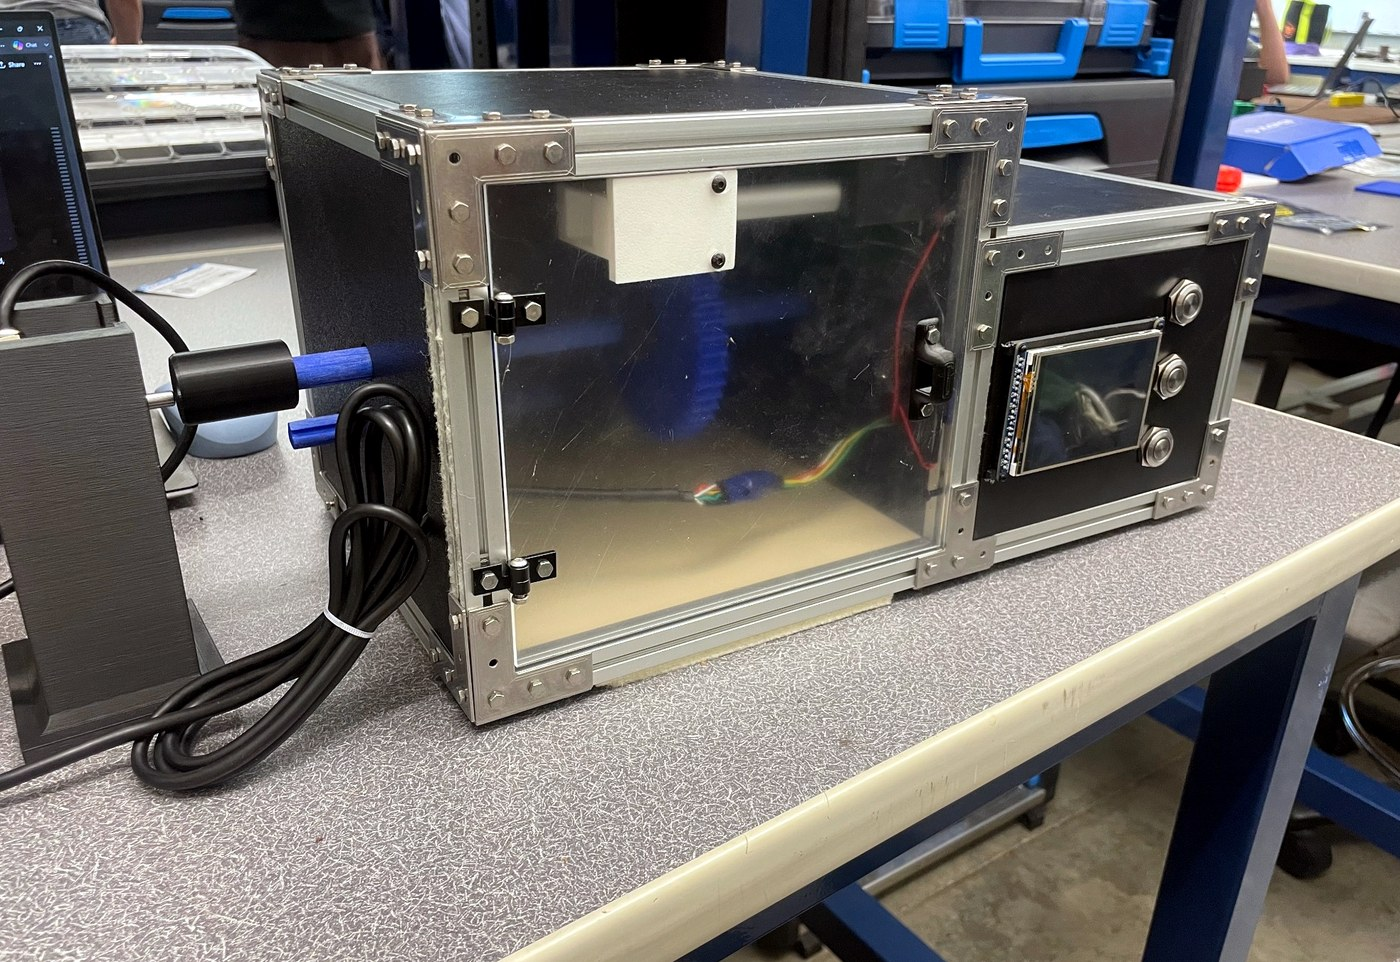
\includegraphics[
        width=5.55in,
        height=2.76in,
        keepaspectratio
    ]{prototype_overview.jpg}
};

\node[
    anchor=north,
    align=center,
    inner sep=0pt,
    text width=5.30in,
    text=Muted,
    font=\sffamily\fontsize{6.25}{6.95}\selectfont
]
at ($(current page.north west)+(7.2in,-4.46in)$)
{Completed gearbox demonstration with enclosed mechanism, TFT interface, and user controls};

% Lower section title
\node[
    anchor=north west,
    text=DeepGreen,
    font=\sffamily\bfseries\fontsize{8.0}{8.7}\selectfont
]
at ($(current page.north west)+(0.43in,-4.70in)$)
{SYSTEM DEVELOPMENT AND FINAL ARCHITECTURE};

% Lower left — CAD card
\node[
    anchor=north west,
    inner sep=2.5pt,
    draw=RuleGray,
    line width=0.55pt,
    rounded corners=5pt
]
at ($(current page.north west)+(0.42in,-4.95in)$)
{
    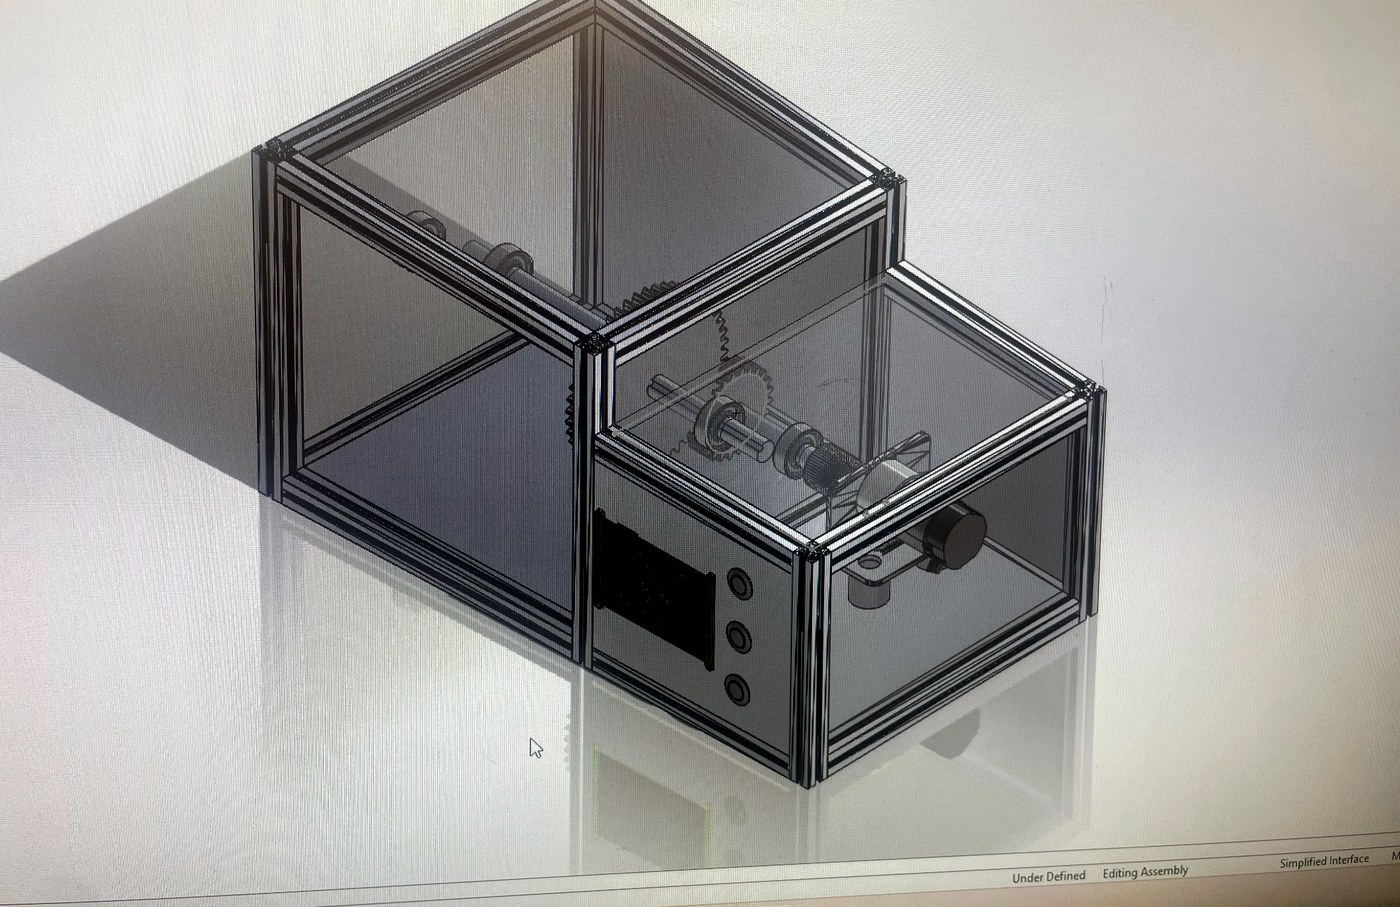
\includegraphics[
        width=2.88in,
        height=1.93in,
        keepaspectratio
    ]{cad_overview.jpg}
};

\node[
    anchor=north,
    align=center,
    inner sep=0pt,
    text width=2.72in,
    text=Muted,
    font=\sffamily\fontsize{6.05}{6.75}\selectfont
]
at ($(current page.north west)+(1.86in,-6.98in)$)
{SolidWorks packaging concept for the gearbox, enclosure, and control panel};

% Lower center — wiring diagram
\node[
    anchor=north west,
    inner sep=2.5pt,
    draw=RuleGray,
    line width=0.55pt,
    rounded corners=5pt
]
at ($(current page.north west)+(3.56in,-4.95in)$)
{
    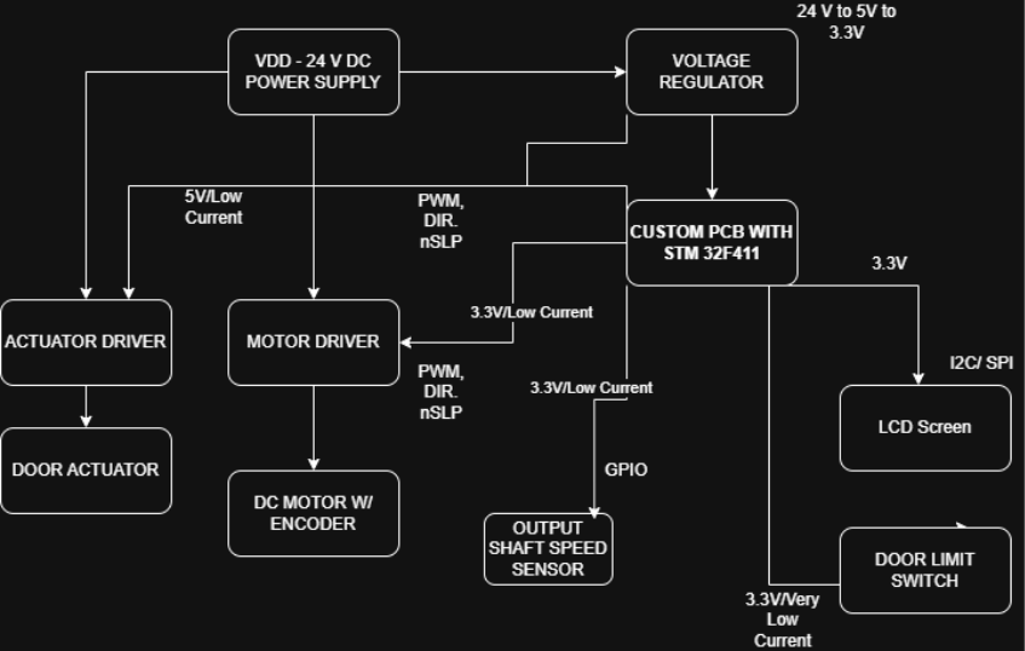
\includegraphics[
        width=3.62in,
        height=1.93in,
        keepaspectratio
    ]{WIRING_DIAGRAM.png}
};

\node[
    anchor=north,
    align=center,
    inner sep=0pt,
    text width=3.46in,
    text=Muted,
    font=\sffamily\fontsize{6.05}{6.75}\selectfont
]
at ($(current page.north west)+(5.37in,-6.98in)$)
{Power and control architecture};

% Lower right — platform highlights moved into the open space
\fill[SoftGreen,rounded corners=5pt]
    ($(current page.north west)+(6.98in,-4.95in)$)
    rectangle
    ($(current page.north east)+(-0.42in,-6.91in)$);

\draw[RuleGray,line width=0.55pt,rounded corners=5pt]
    ($(current page.north west)+(6.98in,-4.95in)$)
    rectangle
    ($(current page.north east)+(-0.42in,-6.91in)$);

\node[
    anchor=north west,
    text=DeepGreen,
    font=\sffamily\bfseries\fontsize{7.75}{8.45}\selectfont
]
at ($(current page.north west)+(7.20in,-5.14in)$)
{PLATFORM HIGHLIGHTS};

\node[
    anchor=north west,
    align=left,
    text width=3.08in,
    text=Ink,
    font=\fontsize{5.72}{6.58}\selectfont
]
at ($(current page.north west)+(7.20in,-5.43in)$)
{
\textbf{Four-layer board.}
Signals were routed on the top and bottom copper layers, with an internal 3.3 V logic plane and a dedicated ground plane.\\[4pt]

\textbf{Integrated control.}
The PCB combines dual encoder inputs, motor and actuator control, a TFT display, user buttons, USB, SWD, voltage sensing, and expansion headers.
};

% Standalone full-width centered resource bar
\fill[Panel,rounded corners=4pt]
    ($(current page.north west)+(0.42in,-7.20in)$)
    rectangle
    ($(current page.north east)+(-0.42in,-7.64in)$);

\draw[RuleGray,line width=0.5pt,rounded corners=4pt]
    ($(current page.north west)+(0.42in,-7.20in)$)
    rectangle
    ($(current page.north east)+(-0.42in,-7.64in)$);

\node[
    anchor=center,
    align=center,
    text=DeepGreen,
    font=\sffamily\bfseries\fontsize{6.75}{7.35}\selectfont
]
at ($(current page.north)+(0,-7.42in)$)
{
\href{\GearMeshVideoURL}{\faPlayCircle\ GEAR MESH DEMO}
\hspace{24pt}
\href{\GearboxSchematicOneURL}{\faFilePdf\ SCHEMATIC 1}
\hspace{24pt}
\href{\GearboxSchematicTwoURL}{\faFilePdf\ SCHEMATIC 2}
};

% Footer
\node[
    anchor=south west,
    text=white,
    font=\sffamily\bfseries\fontsize{7.1}{7.7}\selectfont
]
at ($(current page.south west)+(0.42in,0.17in)$)
{\hyperlink{mechatronics}{\faArrowLeft\ MECHATRONICS}};

\node[
    anchor=south,
    text=white,
    font=\sffamily\fontsize{7.0}{7.6}\selectfont
]
at ($(current page.south)+(0,0.17in)$)
{GEARBOX CONTROLLER \hspace{6pt} 1 / 3};

\node[
    anchor=south east,
    text=white,
    font=\sffamily\bfseries\fontsize{7.1}{7.7}\selectfont
]
at ($(current page.south east)+(-0.42in,0.17in)$)
{PCB ARCHITECTURE \faArrowRight};

\end{tikzpicture}

% ============================================================
% PAGE 2 — PCB DESIGN, ROUTING, AND MANUFACTURING
% Images used on this page:
%   pcb_render.png
%   complete_pcb.jpeg
%   Top_layer.png
%   bottom_layer.png
%   stm32_pinout.png
% Resources used on this page:
%   JLCPCB BOM
%   Pick-and-Place
%   PCB Pinout Logic
% ============================================================

\clearpage
\thispagestyle{empty}
\null

\begin{tikzpicture}[remember picture,overlay]

% Background and bars
\fill[white] (current page.south west) rectangle (current page.north east);

\fill[DeepGreen]
    (current page.north west)
    rectangle
    ($(current page.north east)+(0,-0.095in)$);

\fill[PolyGold]
    ($(current page.north west)+(0,-0.095in)$)
    rectangle
    ($(current page.north east)+(0,-0.14in)$);

\fill[DeepGreen]
    (current page.south west)
    rectangle
    ($(current page.south east)+(0,0.36in)$);

\fill[PolyGold]
    ($(current page.south west)+(0,0.36in)$)
    rectangle
    ($(current page.south east)+(0,0.405in)$);

% Header
\node[
    anchor=north west,
    text=PolyGold,
    font=\sffamily\bfseries\fontsize{8.1}{8.7}\selectfont
]
at ($(current page.north west)+(0.42in,-0.39in)$)
{GEARBOX CONTROLLER \hspace{5pt}/\hspace{5pt} PCB ARCHITECTURE};

\node[
    anchor=north west,
    text=DeepGreen,
    font=\bfseries\fontsize{21.5}{22.5}\selectfont
]
at ($(current page.north west)+(0.40in,-0.67in)$)
{FROM COMPONENT SELECTION TO MANUFACTURED BOARD};

\node[
    anchor=north west,
    text=Muted,
    font=\sffamily\fontsize{8.2}{8.95}\selectfont
]
at ($(current page.north west)+(0.42in,-1.12in)$)
{Independent circuit development, JLCPCB sourcing, multilayer routing, assembly, and embedded hardware integration};

\fill[PolyGold]
    ($(current page.north west)+(0.42in,-1.36in)$)
    rectangle
    ($(current page.north west)+(8.80in,-1.315in)$);

% Top left — populated 3D render
\node[
    anchor=north west,
    inner sep=2.6pt,
    draw=DeepGreen,
    line width=0.68pt,
    rounded corners=5pt
]
at ($(current page.north west)+(0.42in,-1.58in)$)
{
    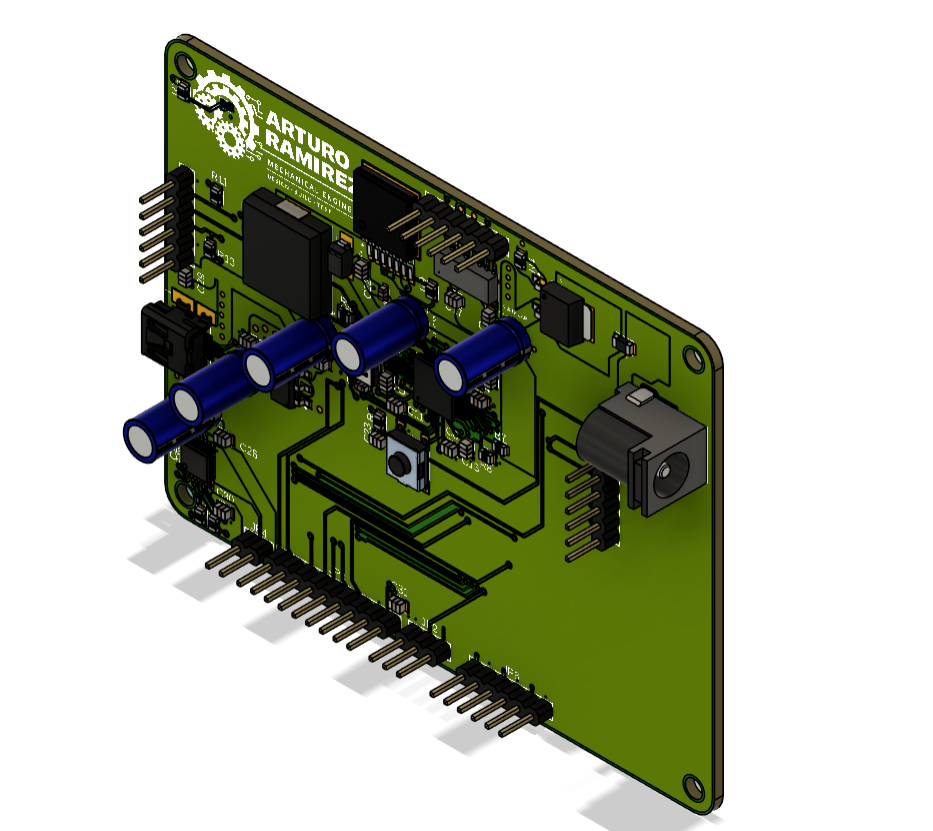
\includegraphics[
        width=3.23in,
        height=2.25in,
        keepaspectratio
    ]{pcb_render.png}
};

\node[
    anchor=north,
    align=center,
    inner sep=0pt,
    text width=3.08in,
    text=Muted,
    font=\sffamily\fontsize{6.15}{6.85}\selectfont
]
at ($(current page.north west)+(1.7in,-3.94in)$)
{Fusion 360 Electronics render of the populated controller PCB};

% Top center — fabricated PCB photograph
\node[
    anchor=north west,
    inner sep=2.6pt,
    draw=DeepGreen,
    line width=0.68pt,
    rounded corners=5pt
]
at ($(current page.north west)+(3.90in,-1.58in)$)
{
    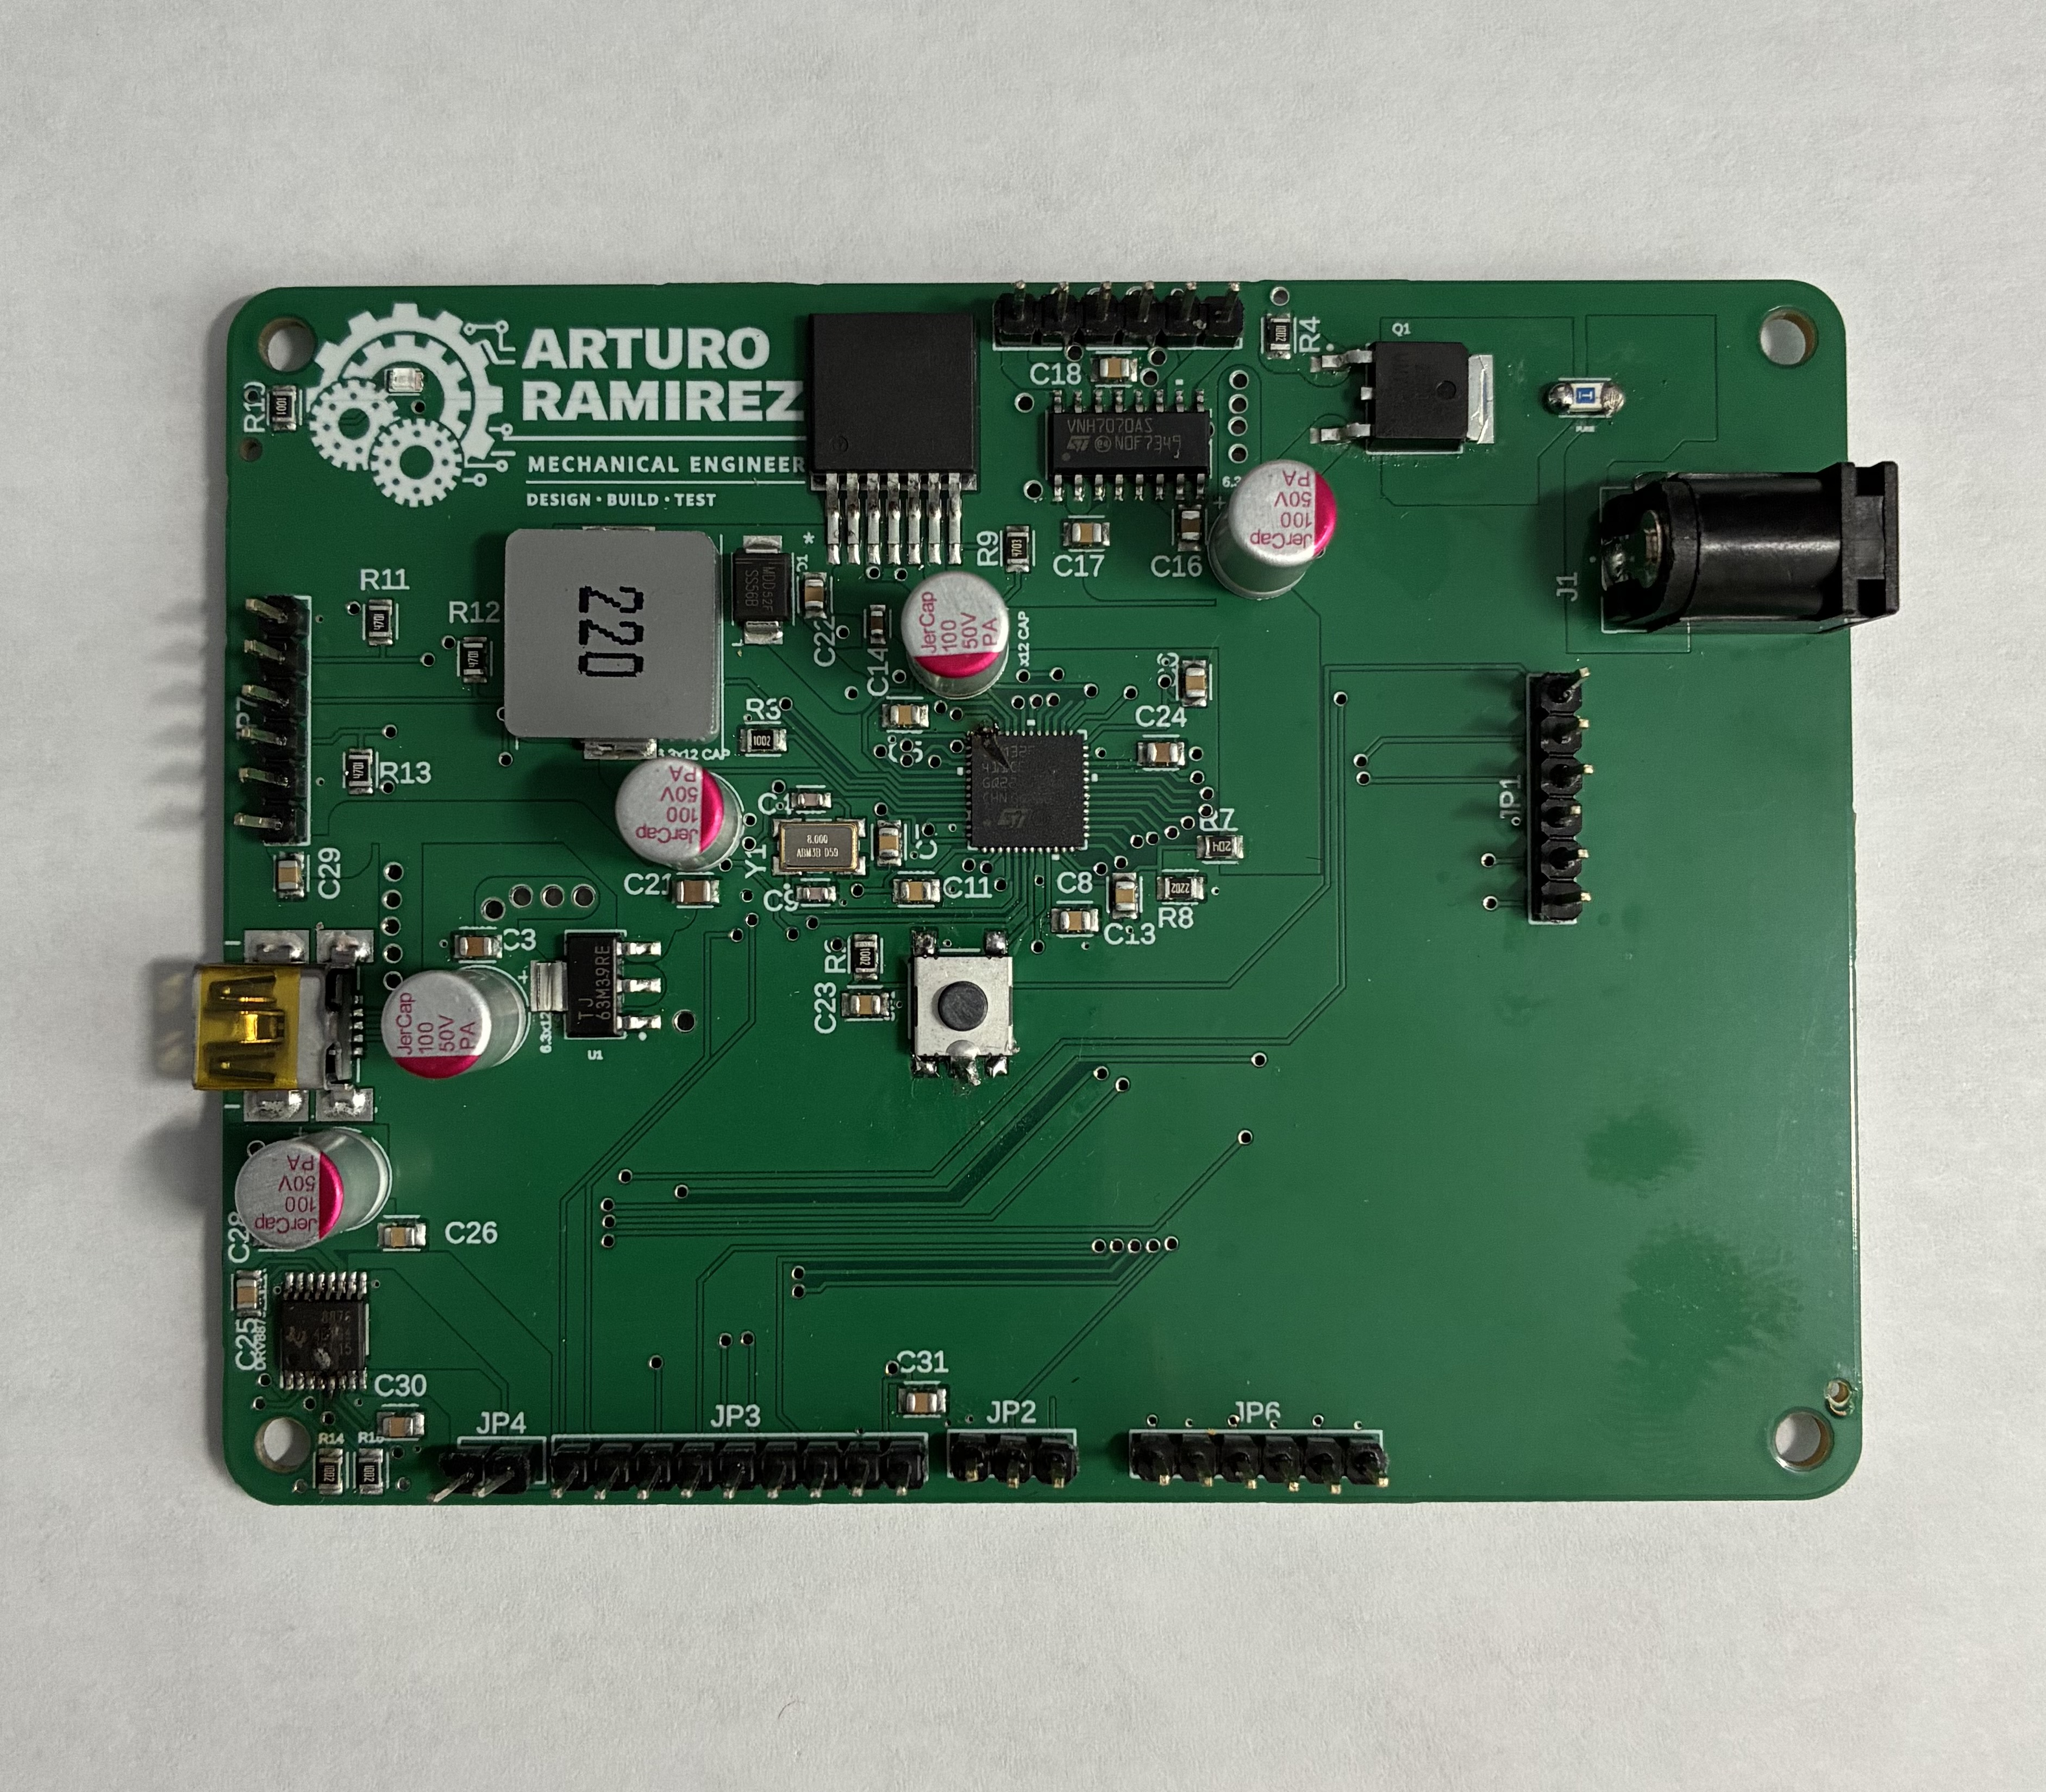
\includegraphics[
        width=3.38in,
        height=2.25in,
        keepaspectratio
    ]{complete_pcb.jpeg}
};

\node[
    anchor=north,
    align=center,
    inner sep=0pt,
    text width=3.20in,
    text=Muted,
    font=\sffamily\fontsize{6.15}{6.85}\selectfont
]
at ($(current page.north west)+(5.2in,-3.94in)$)
{Fabricated and partially populated first-generation controller PCB};

% Top right — design approach
\fill[SoftGold,rounded corners=5pt]
    ($(current page.north west)+(7.52in,-1.58in)$)
    rectangle
    ($(current page.north east)+(-0.42in,-2.71in)$);

\fill[PolyGold]
    ($(current page.north west)+(7.52in,-1.58in)$)
    rectangle
    ($(current page.north west)+(7.62in,-2.71in)$);

\node[
    anchor=north west,
    text=DeepGreen,
    font=\sffamily\bfseries\fontsize{7.8}{8.5}\selectfont
]
at ($(current page.north west)+(7.82in,-1.76in)$)
{DESIGN APPROACH};

\node[
    anchor=north west,
    align=left,
    text width=2.48in,
    text=Ink,
    font=\fontsize{5.30}{6.05}\selectfont
]
at ($(current page.north west)+(7.82in,-2.04in)$)
{
The board was developed from the system requirements outward.\\[2pt]
MCUs, drivers, regulators, connectors, passives, footprints, and
protection devices were verified against datasheets, package limits,
assembly access, and JLCPCB availability before routing.
};

% Top right — integrated features
\fill[SoftGreen,rounded corners=5pt]
    ($(current page.north west)+(7.52in,-2.91in)$)
    rectangle
    ($(current page.north east)+(-0.42in,-4.04in)$);

\draw[RuleGray,line width=0.55pt,rounded corners=5pt]
    ($(current page.north west)+(7.52in,-2.91in)$)
    rectangle
    ($(current page.north east)+(-0.42in,-4.04in)$);

\node[
    anchor=north west,
    text=DeepGreen,
    font=\sffamily\bfseries\fontsize{7.8}{8.5}\selectfont
]
at ($(current page.north west)+(7.78in,-3.09in)$)
{INTEGRATED FEATURES};

\node[
    anchor=north west,
    align=left,
    text width=2.86in,
    text=Ink,
    font=\fontsize{5.55}{6.38}\selectfont
]
at ($(current page.north west)+(7.78in,-3.37in)$)
{
STM32F411 \textbullet\ 24 V input\\
5 V buck \textbullet\ 3.3 V logic\\
Motor and actuator control\\
Dual encoder interfaces\\
SPI TFT \textbullet\ buttons \textbullet\ limit switch\\
USB \textbullet\ SWD \textbullet\ voltage sensing
};

% Routing section title
\node[
    anchor=north west,
    text=DeepGreen,
    font=\sffamily\bfseries\fontsize{8.0}{8.7}\selectfont
]
at ($(current page.north west)+(0.43in,-4.30in)$)
{ROUTING, MCU ASSIGNMENT, AND DESIGN FOR MANUFACTURING};

% Routing cards
\node[
    anchor=north west,
    inner sep=2.4pt,
    draw=RuleGray,
    line width=0.55pt,
    rounded corners=4pt
]
at ($(current page.north west)+(0.42in,-4.56in)$)
{
    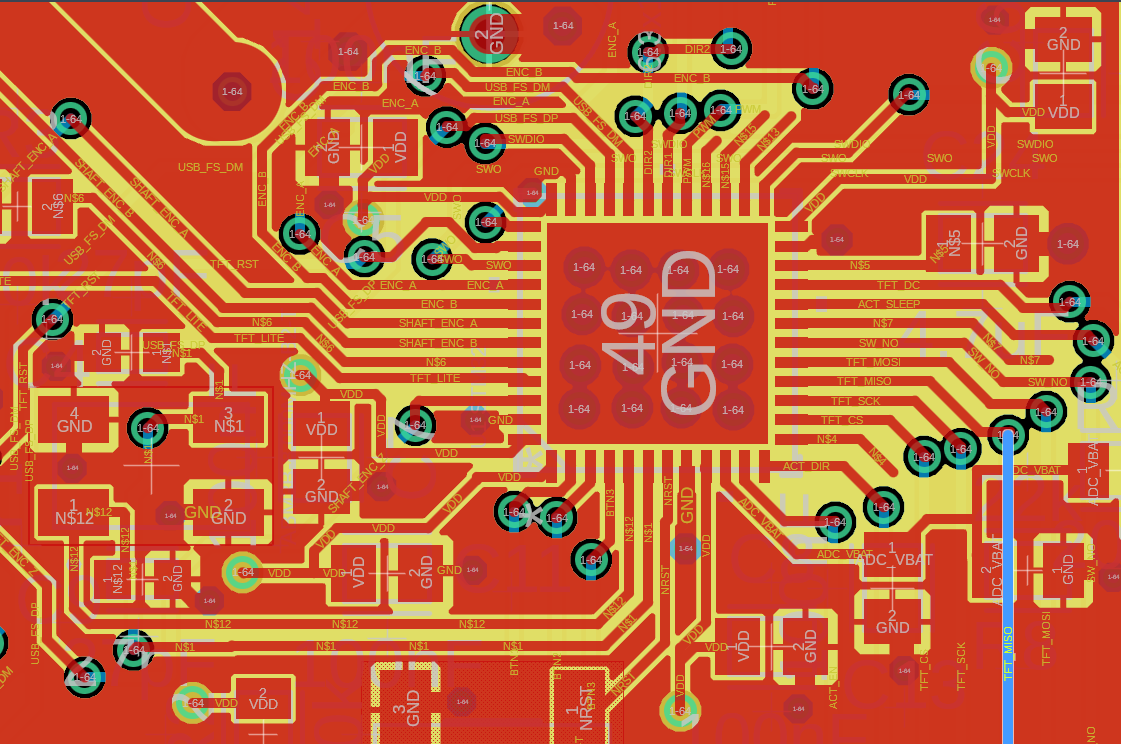
\includegraphics[
        width=3.34in,
        height=1.64in,
        keepaspectratio
    ]{Top_layer.png}
};

\node[
    anchor=north,
    align=center,
    inner sep=0pt,
    text width=3.18in,
    text=Muted,
    font=\sffamily\fontsize{6.10}{6.80}\selectfont
]
at ($(current page.north west)+(1.8in,-6.29in)$)
{Top-layer routing and component fan-out};

\node[
    anchor=north west,
    inner sep=2.4pt,
    draw=RuleGray,
    line width=0.55pt,
    rounded corners=4pt
]
at ($(current page.north west)+(3.98in,-4.56in)$)
{
    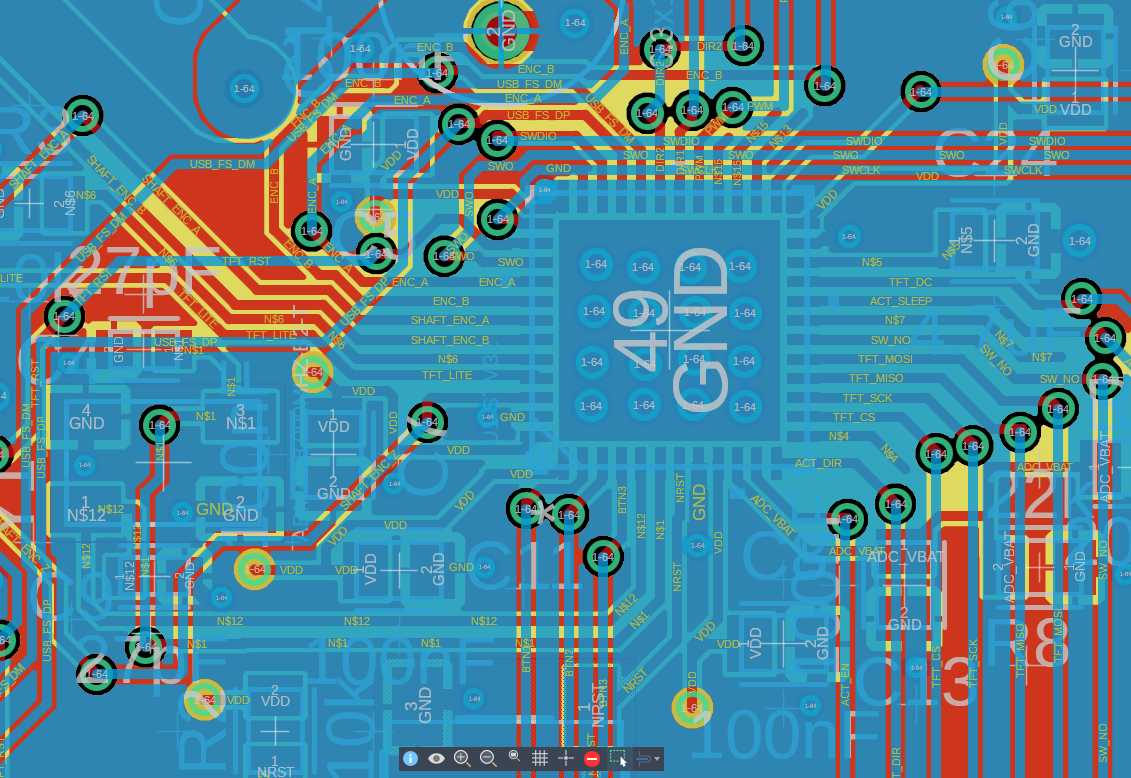
\includegraphics[
        width=3.34in,
        height=1.64in,
        keepaspectratio
    ]{bottom_layer.png}
};

\node[
    anchor=north,
    align=center,
    inner sep=0pt,
    text width=3.18in,
    text=Muted,
    font=\sffamily\fontsize{6.10}{6.80}\selectfont
]
at ($(current page.north west)+(5.3in,-6.29in)$)
{Bottom-layer routing and return-path organization};

\node[
    anchor=north west,
    inner sep=2.4pt,
    draw=RuleGray,
    line width=0.55pt,
    rounded corners=4pt
]
at ($(current page.north west)+(7.54in,-4.56in)$)
{
    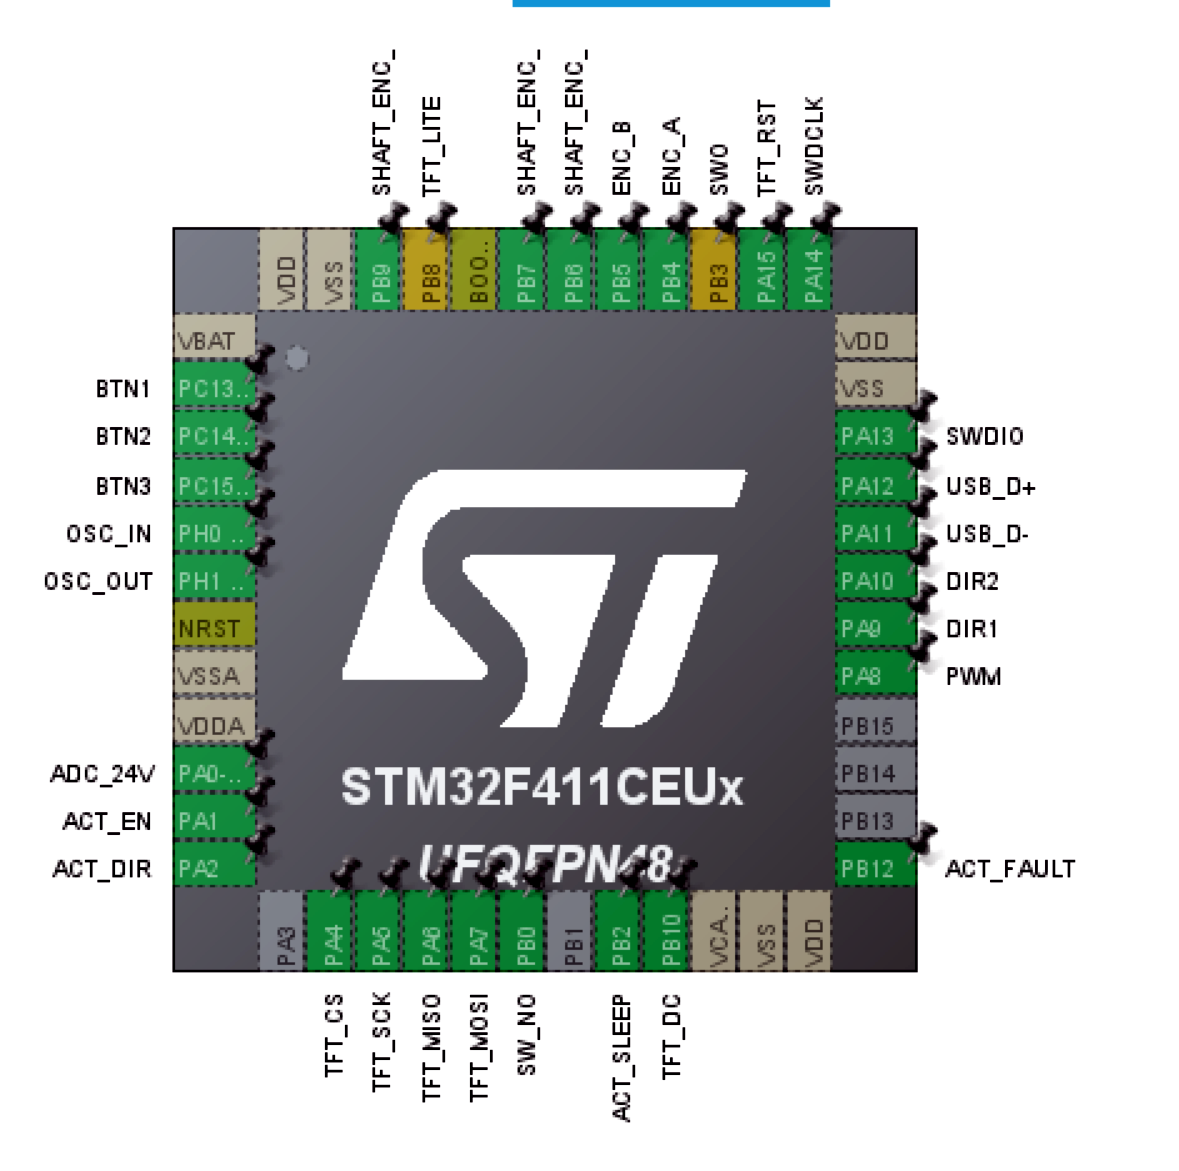
\includegraphics[
        width=3.20in,
        height=1.64in,
        keepaspectratio
    ]{stm32_pinout.png}
};

\node[
    anchor=north,
    align=center,
    inner sep=0pt,
    text width=3.04in,
    text=Muted,
    font=\sffamily\fontsize{6.10}{6.80}\selectfont
]
at ($(current page.north west)+(8.45in,-6.29in)$)
{STM32F411 GPIO and peripheral assignment};

% Bottom engineering panels
\fill[SoftGreen,rounded corners=5pt]
    ($(current page.north west)+(0.42in,-6.56in)$)
    rectangle
    ($(current page.north west)+(5.34in,-7.24in)$);

\draw[RuleGray,line width=0.55pt,rounded corners=5pt]
    ($(current page.north west)+(0.42in,-6.56in)$)
    rectangle
    ($(current page.north west)+(5.34in,-7.24in)$);

\node[
    anchor=north west,
    text=DeepGreen,
    font=\sffamily\bfseries\fontsize{7.25}{7.95}\selectfont
]
at ($(current page.north west)+(0.66in,-6.70in)$)
{POWER ARCHITECTURE};

\node[
    anchor=north west,
    align=left,
    text width=4.40in,
    text=Ink,
    font=\fontsize{6.02}{6.90}\selectfont
]
at ($(current page.north west)+(0.66in,-6.94in)$)
{
24 V motor supply \(\rightarrow\) protected input \(\rightarrow\) 5 V buck conversion
\(\rightarrow\) 3.3 V logic regulation, with local bulk and high-frequency decoupling.
};

\fill[SoftGold,rounded corners=5pt]
    ($(current page.north west)+(5.56in,-6.56in)$)
    rectangle
    ($(current page.north east)+(-0.42in,-7.24in)$);

\fill[PolyGold]
    ($(current page.north west)+(5.56in,-6.56in)$)
    rectangle
    ($(current page.north west)+(5.66in,-7.24in)$);

\node[
    anchor=north west,
    text=DeepGreen,
    font=\sffamily\bfseries\fontsize{7.25}{7.95}\selectfont
]
at ($(current page.north west)+(5.86in,-6.70in)$)
{DESIGN FOR MANUFACTURING};

\node[
    anchor=north west,
    align=left,
    text width=4.60in,
    text=Ink,
    font=\fontsize{6.00}{6.88}\selectfont
]
at ($(current page.north west)+(5.86in,-6.94in)$)
{
JLCPCB stock, assembly orientation, connector access, soldering practicality,
test access, and footprint verification directly shaped the final board.
};

% Resource links
\node[
    anchor=north,
    align=center,
    text=DeepGreen,
    font=\sffamily\bfseries\fontsize{6.75}{7.35}\selectfont
]
at ($(current page.north)+(0,-7.45in)$)
{
\href{\GearboxBOMURL}{\faFilePdf\ JLCPCB BOM}
\hspace{18pt}
\href{\GearboxPnPURL}{\faFilePdf\ PICK-AND-PLACE}
\hspace{18pt}
\href{\GearboxPinoutURL}{\faFilePdf\ PCB PINOUT LOGIC}
};

% Footer
\node[
    anchor=south west,
    text=white,
    font=\sffamily\bfseries\fontsize{7.1}{7.7}\selectfont
]
at ($(current page.south west)+(0.42in,0.17in)$)
{\faArrowLeft\ SYSTEM OVERVIEW};

\node[
    anchor=south,
    text=white,
    font=\sffamily\fontsize{7.0}{7.6}\selectfont
]
at ($(current page.south)+(0,0.17in)$)
{GEARBOX CONTROLLER \hspace{6pt} 2 / 3};

\node[
    anchor=south east,
    text=white,
    font=\sffamily\bfseries\fontsize{7.1}{7.7}\selectfont
]
at ($(current page.south east)+(-0.42in,0.17in)$)
{INTEGRATION \& TAKEAWAYS \faArrowRight};

\end{tikzpicture}

% ============================================================
% PAGE 3 — EMBEDDED INTEGRATION, LESSONS, AND FUTURE PLATFORM
% Image used on this page:
%   pcb_layer_view.png
% No Google Drive resource is repeated on this page.
% ============================================================

\clearpage
\thispagestyle{empty}
\null

\begin{tikzpicture}[remember picture,overlay]

% Background and bars
\fill[white] (current page.south west) rectangle (current page.north east);

\fill[DeepGreen]
    (current page.north west)
    rectangle
    ($(current page.north east)+(0,-0.095in)$);

\fill[PolyGold]
    ($(current page.north west)+(0,-0.095in)$)
    rectangle
    ($(current page.north east)+(0,-0.14in)$);

\fill[DeepGreen]
    (current page.south west)
    rectangle
    ($(current page.south east)+(0,0.36in)$);

\fill[PolyGold]
    ($(current page.south west)+(0,0.36in)$)
    rectangle
    ($(current page.south east)+(0,0.405in)$);

% Header
\node[
    anchor=north west,
    text=PolyGold,
    font=\sffamily\bfseries\fontsize{8.1}{8.7}\selectfont
]
at ($(current page.north west)+(0.42in,-0.39in)$)
{GEARBOX CONTROLLER \hspace{5pt}/\hspace{5pt} INTEGRATION AND ENGINEERING TAKEAWAYS};

\node[
    anchor=north west,
    text=DeepGreen,
    font=\bfseries\fontsize{22.0}{23.0}\selectfont
]
at ($(current page.north west)+(0.40in,-0.67in)$)
{A REUSABLE PLATFORM FOR EMBEDDED CONTROL};

\node[
    anchor=north west,
    text=Muted,
    font=\sffamily\fontsize{8.25}{9.0}\selectfont
]
at ($(current page.north west)+(0.42in,-1.12in)$)
{Hardware assembly, CubeMX configuration, collaborative firmware development, and next-generation expansion};

\fill[PolyGold]
    ($(current page.north west)+(0.42in,-1.36in)$)
    rectangle
    ($(current page.north west)+(8.82in,-1.315in)$);

% Large PCB routing image — only use of this image
\node[
    anchor=north west,
    inner sep=2.6pt,
    draw=DeepGreen,
    line width=0.68pt,
    rounded corners=5pt
]
at ($(current page.north west)+(0.42in,-1.58in)$)
{
    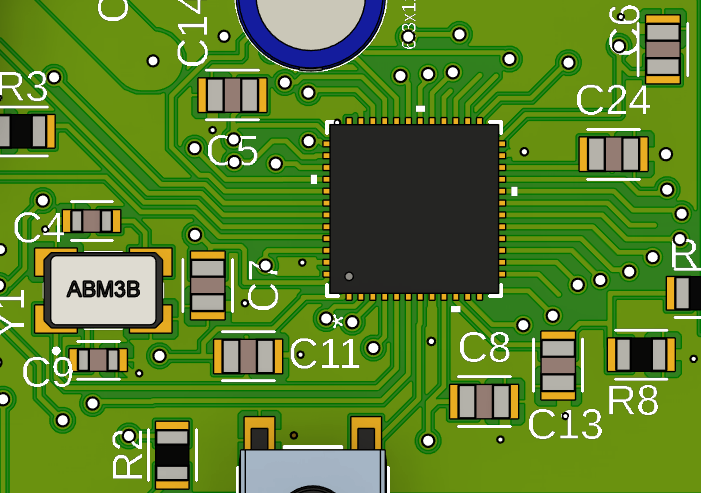
\includegraphics[
        width=5.20in,
        height=3.15in,
        keepaspectratio
    ]{pcb_layer_view.png}
};

\node[
    anchor=north,
    align=center,
    inner sep=0pt,
    text width=4.98in,
    text=Muted,
    font=\sffamily\fontsize{6.30}{7.00}\selectfont
]
at ($(current page.north west)+(3.02in,-4.85in)$)
{Dense MCU breakout, encoder routing, SWD, USB, TFT, actuator, and sensing interfaces};

% Top right — hardware and firmware integration
% Left edge aligned with the Future Learning Platform panel below.
\fill[SoftGold,rounded corners=5pt]
    ($(current page.north west)+(5.56in,-1.58in)$)
    rectangle
    ($(current page.north east)+(-0.42in,-4.92in)$);

\fill[PolyGold]
    ($(current page.north west)+(5.56in,-1.58in)$)
    rectangle
    ($(current page.north west)+(5.66in,-4.92in)$);

\node[
    anchor=north west,
    text=DeepGreen,
    font=\sffamily\bfseries\fontsize{8.0}{8.7}\selectfont
]
at ($(current page.north west)+(5.86in,-1.77in)$)
{HARDWARE AND FIRMWARE INTEGRATION};

\node[
    anchor=north west,
    align=left,
    text width=4.54in,
    text=Ink,
    font=\fontsize{6.65}{7.78}\selectfont
]
at ($(current page.north west)+(5.86in,-2.07in)$)
{
After fabrication, I soldered the selected components and integrated the
PCB into the larger system architecture. My partner and I jointly configured
the STM32 in CubeMX to establish clocking, GPIO, timers, encoder inputs,
SPI communication, USB, and debug access.\\[5pt]

We developed the firmware around collaborative multitasking in C/C++ so
that motor control, display updates, user commands, actuator behavior, and
safety logic could operate as one cohesive controller rather than as isolated
demonstrations.\\[5pt]

This first revision served as a functional learning platform while exposing
practical improvements for protection, test access, connector planning,
packaging, and future instrumentation.
};

% Bottom left — engineering takeaways
\fill[SoftGreen,rounded corners=5pt]
    ($(current page.north west)+(0.42in,-5.18in)$)
    rectangle
    ($(current page.north west)+(5.34in,-7.30in)$);

\draw[RuleGray,line width=0.55pt,rounded corners=5pt]
    ($(current page.north west)+(0.42in,-5.18in)$)
    rectangle
    ($(current page.north west)+(5.34in,-7.30in)$);

\node[
    anchor=north west,
    text=DeepGreen,
    font=\sffamily\bfseries\fontsize{7.8}{8.5}\selectfont
]
at ($(current page.north west)+(0.68in,-5.36in)$)
{ENGINEERING TAKEAWAYS};

\node[
    anchor=north west,
    align=left,
    text width=4.42in,
    text=Ink,
    font=\fontsize{6.25}{7.25}\selectfont
]
at ($(current page.north west)+(0.68in,-5.65in)$)
{
\textbf{Architecture first.}
Defining interfaces before routing reduced late-stage changes and simplified integration.\\[4pt]

\textbf{Datasheets are the design language.}
Selection required verifying voltage, current, package, thermal, and control requirements rather than relying on names alone.\\[4pt]

\textbf{Manufacturability shapes electronics.}
Stock, assembly, access, solderability, and testability directly influenced the final circuit.\\[4pt]

\textbf{First revisions are learning tools.}
Bring-up revealed improvements for protection, debug access, and packaging.
};

% Bottom right — future platform
\fill[SoftGold,rounded corners=5pt]
    ($(current page.north west)+(5.56in,-5.18in)$)
    rectangle
    ($(current page.north east)+(-0.42in,-7.30in)$);

\fill[PolyGold]
    ($(current page.north west)+(5.56in,-5.18in)$)
    rectangle
    ($(current page.north west)+(5.66in,-7.30in)$);

\node[
    anchor=north west,
    text=DeepGreen,
    font=\sffamily\bfseries\fontsize{7.8}{8.5}\selectfont
]
at ($(current page.north west)+(5.86in,-5.36in)$)
{FUTURE LEARNING PLATFORM};

\node[
    anchor=north west,
    align=left,
    text width=4.58in,
    text=Ink,
    font=\fontsize{6.25}{7.25}\selectfont
]
at ($(current page.north west)+(5.86in,-5.65in)$)
{
The controller was intentionally conceived as more than a single-purpose
gearbox driver. Future revisions can add torque sensing, motor-current
measurement, temperature monitoring, improved output-speed sensing,
and additional analog or digital sensors.\\[5pt]

Those additions would support system identification, efficiency studies,
closed-loop speed control, comparison between predicted and measured
gear ratios, and the development of kinetic as well as kinematic models.
The existing PCB, enclosure, display, and modular mechanical platform
provide the foundation for those experiments.
};

% Footer
\node[
    anchor=south west,
    text=white,
    font=\sffamily\bfseries\fontsize{7.1}{7.7}\selectfont
]
at ($(current page.south west)+(0.42in,0.17in)$)
{\faArrowLeft\ PCB ARCHITECTURE};

\node[
    anchor=south,
    text=white,
    font=\sffamily\fontsize{7.0}{7.6}\selectfont
]
at ($(current page.south)+(0,0.17in)$)
{GEARBOX CONTROLLER \hspace{6pt} 3 / 3};

\node[
    anchor=south east,
    text=white,
    font=\sffamily\bfseries\fontsize{7.1}{7.7}\selectfont
]
at ($(current page.south east)+(-0.42in,0.17in)$)
{NEXT PROJECT \faArrowRight};

\end{tikzpicture}


% ============================================================
% ROMI AUTONOMOUS DIFFERENTIAL-DRIVE ROBOT
% FIVE-PAGE PORTFOLIO CASE STUDY
% 02 Mechatronics / Project 07
%
% IMPORTANT
% ----------
% 1. This file is intended to be included from the main portfolio:
%       \input{romi}
%    It must NOT contain \documentclass, \begin{document}, or \end{document}.
%
% 2. The main preamble should already define:
%       DeepGreen, PolyGold, SoftGold, SoftGreen,
%       RuleGray, Muted, Ink, Panel
%    and load:
%       tikz, graphicx, hyperref, fontawesome5, amsmath, amssymb
%
% 3. Upload the following image files to Overleaf using these exact
%    base filenames. Extensions may be .png, .jpg, or .jpeg; LaTeX will
%    resolve them automatically when only the base filename is supplied.
%
%       Romi Hero Image
%       Romi Pluggedin
%       Romi Side View
%       Romi Top View
%       Real Time Software Diagram
%       Chassis Dynamics
%       Dynamics
%       Romi Total Dynamics
%       Wheel Encoder Rotation
%       effort based position
%       effort based velocity
%       gain calibration
%       nested control loop
%       Track Course
%
%    Each image is used only once in this script.
%
% 4. The instructor's timer auto-reload visualization is intentionally
%    excluded because the page prioritizes team-created engineering artifacts.
%
% 5. The notebook HTML button should only be restored after the file has
%    been uploaded to a public HTTPS address. Local file:/// and run: links
%    are intentionally excluded because they break for other viewers.
%
% 6. Resource links are each used once across the five pages.
% ============================================================

% ------------------------------------------------------------
% PROJECT RESOURCE URLS
% ------------------------------------------------------------

\providecommand{\RomiGitHubURL}
{https://github.com/shwanpla/ME-405-Term-Project}

\providecommand{\RomiDocumentationURL}
{https://me-405-term-project.readthedocs.io/en/latest/overview.html}

\providecommand{\RomiTrackYouTubeURL}
{https://youtu.be/gsIIfVX_UOE?si=vdGteQbXHBkoHcBp}

\providecommand{\RomiLineYouTubeURL}
{https://youtu.be/3hr3dCyPbDM?si=kXSeATZV6t0dCAKc}

\providecommand{\RomiDataCaptureURL}
{https://drive.google.com/file/d/1NIpuxDYtf03tbfd8yQCP5n-v_P9-T6j7/view?usp=drive_link}

% Replace this placeholder with the HTML-export link supplied for the project.
% IMPORTANT: A file:///D:/... path is private to one computer and cannot
% be opened by employers. Upload HW0x04_ARTURO_RAMIREZ.html to a public host
% such as GitHub Pages, Google Drive with public access, or a personal website,
% then replace the URL below with that absolute https:// address.
%
% Example after enabling GitHub Pages:
% https://YOUR-USERNAME.github.io/YOUR-REPOSITORY/HW0x04_ARTURO_RAMIREZ.html
%
% Until a public URL is supplied, the notebook button is intentionally omitted
% from the resource row so the portfolio contains no broken link.
\providecommand{\RomiNotebookHTMLURL}
{https://art675.github.io/Romi-Dynamics-Study/}

% ============================================================
% PAGE 1 — SYSTEM OVERVIEW AND PHYSICAL INTEGRATION
% ============================================================

\clearpage
\thispagestyle{empty}
\hypertarget{romi}{}
\null

\begin{tikzpicture}[remember picture,overlay]

% Background and page bars
\fill[white] (current page.south west) rectangle (current page.north east);

\fill[DeepGreen]
    (current page.north west)
    rectangle
    ($(current page.north east)+(0,-0.095in)$);

\fill[PolyGold]
    ($(current page.north west)+(0,-0.095in)$)
    rectangle
    ($(current page.north east)+(0,-0.14in)$);

\fill[DeepGreen]
    (current page.south west)
    rectangle
    ($(current page.south east)+(0,0.36in)$);

\fill[PolyGold]
    ($(current page.south west)+(0,0.36in)$)
    rectangle
    ($(current page.south east)+(0,0.405in)$);

% Header
\node[
    anchor=north west,
    text=PolyGold,
    font=\sffamily\bfseries\fontsize{8.1}{8.7}\selectfont
]
at ($(current page.north west)+(0.42in,-0.39in)$)
{02 MECHATRONICS \hspace{5pt}/\hspace{5pt} PROJECT 07};

\node[
    anchor=north west,
    text=DeepGreen,
    font=\bfseries\fontsize{22.4}{23.4}\selectfont
]
at ($(current page.north west)+(0.40in,-0.67in)$)
{ROMI AUTONOMOUS DIFFERENTIAL-DRIVE ROBOT};

\node[
    anchor=north west,
    text=Muted,
    font=\sffamily\fontsize{8.25}{9.0}\selectfont
]
at ($(current page.north west)+(0.42in,-1.12in)$)
{Cal Poly Mechatronics Laboratory
\hspace{7pt}\textbullet\hspace{7pt}
Three-Person Team
\hspace{7pt}\textbullet\hspace{7pt}
Fall 2025
\hspace{7pt}\textbullet\hspace{7pt}
San Luis Obispo, California};

\fill[PolyGold]
    ($(current page.north west)+(0.42in,-1.36in)$)
    rectangle
    ($(current page.north west)+(8.90in,-1.315in)$);

% Hero image
\node[
    anchor=north west,
    inner sep=2.7pt,
    draw=DeepGreen,
    line width=0.70pt,
    rounded corners=6pt
]
at ($(current page.north west)+(0.42in,-1.58in)$)
{
    \includegraphics[
        width=5.18in,
        height=3.26in,
        keepaspectratio
    ]{\detokenize{Romi Hero Image}}
};

\node[
    anchor=north,
    align=center,
    inner sep=0pt,
    text width=4.95in,
    text=Muted,
    font=\sffamily\fontsize{6.30}{7.00}\selectfont
]
at ($(current page.north west)+(3.01in,-4.94in)$)
{Final Romi autonomous robot.};

% Project overview
% Extended farther left while preserving the original 0.10 in accent strip.
\fill[SoftGold,rounded corners=5pt]
    ($(current page.north west)+(4.43in,-1.58in)$)
    rectangle
    ($(current page.north east)+(-0.42in,-4.98in)$);

\fill[PolyGold]
    ($(current page.north west)+(4.43in,-1.58in)$)
    rectangle
    ($(current page.north west)+(4.53in,-4.98in)$);

\node[
    anchor=north west,
    text=DeepGreen,
    font=\sffamily\bfseries\fontsize{8.0}{8.7}\selectfont
]
at ($(current page.north west)+(4.73in,-1.76in)$)
{PROJECT OVERVIEW};

\node[
    anchor=north west,
    align=left,
    text width=5.73in,
    text=Ink,
    font=\fontsize{6.45}{7.50}\selectfont
]
at ($(current page.north west)+(4.73in,-2.05in)$)
{
Our three-person team built a fully integrated autonomous differential-drive
robot for a course-specific navigation challenge. The system combined an
STM32 Nucleo running MicroPython, wheel encoders, a QTR reflectance array,
a BNO055 IMU, bumper sensing, Bluetooth/serial telemetry, and closed-loop
motor control.\\[4pt]

The software architecture separated hardware drivers, periodic sensing,
state estimation, velocity control, data processing, communications, and
navigation into cooperative generator-based tasks. Shared variables and
queues provided explicit interfaces between subsystems while a priority-based
scheduler maintained deterministic update periods.\\[4pt]

Programming, dynamic analysis, controller tuning, testing, and integration
were shared across the team. The project emphasized collaborative code
development rather than isolated subsystem ownership.
};

\node[
    anchor=south west,
    text=PolyGold,
    font=\sffamily\bfseries\fontsize{6.25}{6.95}\selectfont
]
at ($(current page.north west)+(4.73in,-4.82in)$)
{MICROPYTHON \hspace{6pt}\textbullet\hspace{6pt}
STM32 \hspace{6pt}\textbullet\hspace{6pt}
COOPERATIVE MULTITASKING \hspace{6pt}\textbullet\hspace{6pt}
CLOSED-LOOP CONTROL};

% Supporting hardware images
\node[
    anchor=north west,
    text=DeepGreen,
    font=\sffamily\bfseries\fontsize{8.0}{8.7}\selectfont
]
at ($(current page.north west)+(0.43in,-5.22in)$)
{HARDWARE BRING-UP AND SENSOR INTEGRATION};

% Equal-width light-green image cards
\fill[SoftGreen!46,rounded corners=5pt]
    ($(current page.north west)+(0.42in,-5.48in)$)
    rectangle
    ($(current page.north west)+(3.63in,-7.18in)$);

\draw[RuleGray,line width=0.55pt,rounded corners=5pt]
    ($(current page.north west)+(0.42in,-5.48in)$)
    rectangle
    ($(current page.north west)+(3.63in,-7.18in)$);

\fill[SoftGreen!46,rounded corners=5pt]
    ($(current page.north west)+(4.05in,-5.48in)$)
    rectangle
    ($(current page.north west)+(7.26in,-7.18in)$);

\draw[RuleGray,line width=0.55pt,rounded corners=5pt]
    ($(current page.north west)+(4.05in,-5.48in)$)
    rectangle
    ($(current page.north west)+(7.26in,-7.18in)$);

\fill[SoftGreen!46,rounded corners=5pt]
    ($(current page.north west)+(7.46in,-5.48in)$)
    rectangle
    ($(current page.north west)+(10.67in,-7.18in)$);

\draw[RuleGray,line width=0.55pt,rounded corners=5pt]
    ($(current page.north west)+(7.46in,-5.48in)$)
    rectangle
    ($(current page.north west)+(10.67in,-7.18in)$);

% Card 1 — firmware flashing
\node[
    anchor=north,
    inner sep=2.2pt,
    draw=RuleGray,
    line width=0.50pt,
    rounded corners=3pt,
    fill=white
]
at ($(current page.north west)+(2.025in,-5.61in)$)
{
    \includegraphics[
        width=2.82in,
        height=1.17in,
        keepaspectratio
    ]{\detokenize{Romi Pluggedin}}
};

\node[
    anchor=north,
    align=center,
    text width=2.78in,
    text=Muted,
    font=\sffamily\fontsize{6.25}{6.85}\selectfont
]
at ($(current page.north west)+(2.025in,-6.91in)$)
{Firmware flashing};

% Card 2 — side view
\node[
    anchor=north,
    inner sep=2.2pt,
    draw=RuleGray,
    line width=0.50pt,
    rounded corners=3pt,
    fill=white
]
at ($(current page.north west)+(5.655in,-5.61in)$)
{
    \includegraphics[
        width=2.82in,
        height=1.17in,
        keepaspectratio
    ]{\detokenize{Romi Side View}}
};

\node[
    anchor=north,
    align=center,
    text width=2.78in,
    text=Muted,
    font=\sffamily\fontsize{6.25}{6.85}\selectfont
]
at ($(current page.north west)+(5.655in,-6.91in)$)
{Side view};

% Card 3 — top view
\node[
    anchor=north,
    inner sep=2.2pt,
    draw=RuleGray,
    line width=0.50pt,
    rounded corners=3pt,
    fill=white
]
at ($(current page.north west)+(9.065in,-5.61in)$)
{
    \includegraphics[
        width=2.82in,
        height=1.17in,
        keepaspectratio
    ]{\detokenize{Romi Top View}}
};

\node[
    anchor=north,
    align=center,
    text width=2.78in,
    text=Muted,
    font=\sffamily\fontsize{6.25}{6.85}\selectfont
]
at ($(current page.north west)+(9.065in,-6.91in)$)
{Top view};

% Footer
\node[
    anchor=south west,
    text=white,
    font=\sffamily\bfseries\fontsize{7.1}{7.7}\selectfont
]
at ($(current page.south west)+(0.42in,0.17in)$)
{\hyperlink{gearboxpcb}{\faArrowLeft\ GEARBOX CONTROLLER}};

\node[
    anchor=south,
    text=white,
    font=\sffamily\fontsize{7.0}{7.6}\selectfont
]
at ($(current page.south)+(0,0.17in)$)
{ROMI AUTONOMOUS ROBOT \hspace{6pt} 1 / 5};

\node[
    anchor=south east,
    text=white,
    font=\sffamily\bfseries\fontsize{7.1}{7.7}\selectfont
]
at ($(current page.south east)+(-0.42in,0.17in)$)
{SOFTWARE ARCHITECTURE \faArrowRight};

\end{tikzpicture}

% ============================================================
% PAGE 2 — REAL-TIME SOFTWARE ARCHITECTURE
% ============================================================

\clearpage
\thispagestyle{empty}
\null

\begin{tikzpicture}[remember picture,overlay]

\fill[white] (current page.south west) rectangle (current page.north east);
\fill[DeepGreen] (current page.north west) rectangle ($(current page.north east)+(0,-0.095in)$);
\fill[PolyGold] ($(current page.north west)+(0,-0.095in)$) rectangle ($(current page.north east)+(0,-0.14in)$);
\fill[DeepGreen] (current page.south west) rectangle ($(current page.south east)+(0,0.36in)$);
\fill[PolyGold] ($(current page.south west)+(0,0.36in)$) rectangle ($(current page.south east)+(0,0.405in)$);

\node[
    anchor=north west,
    text=PolyGold,
    font=\sffamily\bfseries\fontsize{8.1}{8.7}\selectfont
]
at ($(current page.north west)+(0.42in,-0.39in)$)
{ROMI AUTONOMOUS ROBOT \hspace{5pt}/\hspace{5pt} REAL-TIME SOFTWARE};

\node[
    anchor=north west,
    text=DeepGreen,
    font=\bfseries\fontsize{22.0}{23.0}\selectfont
]
at ($(current page.north west)+(0.40in,-0.67in)$)
{COOPERATIVE TASK ARCHITECTURE AND DATA FLOW};

\node[
    anchor=north west,
    text=Muted,
    font=\sffamily\fontsize{8.25}{9.0}\selectfont
]
at ($(current page.north west)+(0.42in,-1.12in)$)
{Generator-based tasks, shared variables, queues, priorities, periods, and finite-state navigation};

\fill[PolyGold]
    ($(current page.north west)+(0.42in,-1.36in)$)
    rectangle
    ($(current page.north west)+(8.72in,-1.315in)$);

% Main architecture image
\node[
    anchor=north west,
    inner sep=2.8pt,
    draw=DeepGreen,
    line width=0.68pt,
    rounded corners=5pt
]
at ($(current page.north west)+(0.42in,-1.58in)$)
{
    \includegraphics[
        width=6.74in,
        height=5.55in,
        keepaspectratio
    ]{\detokenize{Real Time Software Diagram}}
};

\node[
    anchor=north,
    align=center,
    text width=6.45in,
    text=Muted,
    font=\sffamily\fontsize{6.25}{6.95}\selectfont
]
at ($(current page.north west)+(3.79in,-7.25in)$)
{Team-developed real-time task diagram showing priorities, periods, shared data, commands, and telemetry paths};

% Architecture explanation
\fill[SoftGold,rounded corners=5pt]
    ($(current page.north west)+(6.62in,-1.58in)$)
    rectangle
    ($(current page.north east)+(-0.42in,-3.58in)$);

\fill[PolyGold]
    ($(current page.north west)+(6.62in,-1.58in)$)
    rectangle
    ($(current page.north west)+(6.72in,-3.58in)$);

\node[
    anchor=north west,
    text=DeepGreen,
    font=\sffamily\bfseries\fontsize{7.8}{8.5}\selectfont
]
at ($(current page.north west)+(7.00in,-1.76in)$)
{WHY THE ARCHITECTURE MATTERED};

\node[
    anchor=north west,
    align=left,
    text width=3.28in,
    text=Ink,
    font=\fontsize{5.52}{6.34}\selectfont
]
at ($(current page.north west)+(6.96in,-2.05in)$)
{
Each subsystem ran as a periodic generator task rather than as one
monolithic loop. This kept sensing, estimation, control, navigation,
data logging, and communications independently testable while preserving
deterministic update timing.\\[3.5pt]

Queues carried ordered data streams; shared variables exposed the latest
state or command; object interfaces encapsulated hardware drivers.
};

% Software stack
\fill[SoftGreen,rounded corners=5pt]
    ($(current page.north west)+(6.62in,-3.82in)$)
    rectangle
    ($(current page.north east)+(-0.42in,-5.53in)$);

\draw[RuleGray,line width=0.55pt,rounded corners=5pt]
    ($(current page.north west)+(6.62in,-3.82in)$)
    rectangle
    ($(current page.north east)+(-0.42in,-5.53in)$);

\node[
    anchor=north west,
    text=DeepGreen,
    font=\sffamily\bfseries\fontsize{7.8}{8.5}\selectfont
]
at ($(current page.north west)+(6.88in,-4.00in)$)
{SOFTWARE STACK};

\node[
    anchor=north west,
    align=left,
    text width=3.56in,
    text=Ink,
    font=\fontsize{5.68}{6.50}\selectfont
]
at ($(current page.north west)+(6.88in,-4.28in)$)
{
\textbf{High level:} main scheduler, navigation FSM, user commands\\[3pt]
\textbf{Middle level:} control, observer, data processing, serial tasks\\[3pt]
\textbf{Low level:} motors, encoders, ADC, I\textsuperscript{2}C IMU, bump and line sensors\\[3pt]
\textbf{Interfaces:} Bluetooth/USB telemetry, reusable classes, explicit task boundaries
};

% Timing panel
\fill[SoftGold,rounded corners=5pt]
    ($(current page.north west)+(6.62in,-5.77in)$)
    rectangle
    ($(current page.north east)+(-0.42in,-7.12in)$);

\fill[PolyGold]
    ($(current page.north west)+(6.62in,-5.77in)$)
    rectangle
    ($(current page.north west)+(6.72in,-7.12in)$);

\node[
    anchor=north west,
    text=DeepGreen,
    font=\sffamily\bfseries\fontsize{7.8}{8.5}\selectfont
]
at ($(current page.north west)+(6.92in,-5.95in)$)
{IMPLEMENTATION DISCIPLINE};

\node[
    anchor=north west,
    align=left,
    text width=3.52in,
    text=Ink,
    font=\fontsize{5.72}{6.54}\selectfont
]
at ($(current page.north west)+(6.92in,-6.23in)$)
{
Tasks were assigned explicit priorities and periods according to control
bandwidth and I/O demands. Incremental integration, serial telemetry, and
repeatable trials made timing errors, stale data, state-transition faults,
and gain interactions visible early.
};

% Resource links
\node[
    anchor=north,
    align=center,
    text=DeepGreen,
    font=\sffamily\bfseries\fontsize{6.75}{7.35}\selectfont
]
at ($(current page.north)+(0,-7.48in)$)
{
\href{\RomiGitHubURL}{\faGithub\ SOURCE CODE}
\hspace{22pt}
\href{\RomiDocumentationURL}{\faBook\ DOCUMENTATION}
};

% Footer
\node[
    anchor=south west,
    text=white,
    font=\sffamily\bfseries\fontsize{7.1}{7.7}\selectfont
]
at ($(current page.south west)+(0.42in,0.17in)$)
{\faArrowLeft\ SYSTEM OVERVIEW};

\node[
    anchor=south,
    text=white,
    font=\sffamily\fontsize{7.0}{7.6}\selectfont
]
at ($(current page.south)+(0,0.17in)$)
{ROMI AUTONOMOUS ROBOT \hspace{6pt} 2 / 5};

\node[
    anchor=south east,
    text=white,
    font=\sffamily\bfseries\fontsize{7.1}{7.7}\selectfont
]
at ($(current page.south east)+(-0.42in,0.17in)$)
{DYNAMIC MODELING \faArrowRight};

\end{tikzpicture}

% ============================================================
% PAGE 3 — DIFFERENTIAL-DRIVE DYNAMICS AND STATE MODELING
% ============================================================

\clearpage
\thispagestyle{empty}
\null

\begin{tikzpicture}[remember picture,overlay]

\fill[white] (current page.south west) rectangle (current page.north east);
\fill[DeepGreen] (current page.north west) rectangle ($(current page.north east)+(0,-0.095in)$);
\fill[PolyGold] ($(current page.north west)+(0,-0.095in)$) rectangle ($(current page.north east)+(0,-0.14in)$);
\fill[DeepGreen] (current page.south west) rectangle ($(current page.south east)+(0,0.36in)$);
\fill[PolyGold] ($(current page.south west)+(0,0.36in)$) rectangle ($(current page.south east)+(0,0.405in)$);

\node[
    anchor=north west,
    text=PolyGold,
    font=\sffamily\bfseries\fontsize{8.1}{8.7}\selectfont
]
at ($(current page.north west)+(0.42in,-0.39in)$)
{ROMI AUTONOMOUS ROBOT \hspace{5pt}/\hspace{5pt} DYNAMIC MODELING};

\node[
    anchor=north west,
    text=DeepGreen,
    font=\bfseries\fontsize{21.6}{22.6}\selectfont
]
at ($(current page.north west)+(0.40in,-0.67in)$)
{FROM WHEEL MOTION TO NONLINEAR ROBOT DYNAMICS};

\node[
    anchor=north west,
    text=Muted,
    font=\sffamily\fontsize{8.15}{8.9}\selectfont
]
at ($(current page.north west)+(0.42in,-1.12in)$)
{Differential-drive kinematics, state selection, first-order motor dynamics, and observer-oriented modeling};

\fill[PolyGold]
    ($(current page.north west)+(0.42in,-1.36in)$)
    rectangle
    ($(current page.north west)+(9.25in,-1.315in)$);

% Kinematics images
\node[
    anchor=north west,
    inner sep=2.4pt,
    draw=RuleGray,
    line width=0.55pt,
    rounded corners=4pt
]
at ($(current page.north west)+(0.42in,-1.58in)$)
{
    \includegraphics[
        width=3.78in,
        height=2.30in,
        keepaspectratio
    ]{\detokenize{Chassis Dynamics}}
};

\node[
    anchor=north west,
    inner sep=2.4pt,
    draw=RuleGray,
    line width=0.55pt,
    rounded corners=4pt
]
at ($(current page.north west)+(4.42in,-1.58in)$)
{
    \includegraphics[
        width=3.78in,
        height=2.30in,
        keepaspectratio
    ]{\detokenize{Dynamics}}
};

\node[
    anchor=north west,
    inner sep=2.4pt,
    draw=RuleGray,
    line width=0.55pt,
    rounded corners=4pt
]
at ($(current page.north west)+(8.43in,-1.58in)$)
{
    \includegraphics[
        width=3.32in,
        height=2.08in,
        keepaspectratio
    ]{\detokenize{Romi Total Dynamics}}
};

\node[
    anchor=north,
    align=center,
    text width=3.55in,
    text=Muted,
    font=\sffamily\fontsize{6.0}{6.7}\selectfont
]
at ($(current page.north west)+(2.31in,-3.81in)$)
{Wheel-speed difference determines yaw rate};

\node[
    anchor=north,
    align=center,
    text width=3.55in,
    text=Muted,
    font=\sffamily\fontsize{6.0}{6.7}\selectfont
]
at ($(current page.north west)+(6.31in,-3.81in)$)
{Wheel-speed average determines forward speed};

\node[
    anchor=north,
    align=center,
    text width=3.10in,
    text=Muted,
    font=\sffamily\fontsize{6.0}{6.7}\selectfont
]
at ($(current page.north west)+(9.7in,-3.81in)$)
{Body velocity mapped into the global frame};

% State vector approach image
% Enlarged while preserving top-edge alignment with the nonlinear model panel.
\node[
    anchor=north west,
    inner sep=2.5pt,
    draw=DeepGreen,
    line width=0.65pt,
    rounded corners=5pt
]
at ($(current page.north west)+(0.42in,-4.03in)$)
{
    \includegraphics[
        width=3.58in,
        height=2.10in,
        keepaspectratio
    ]{\detokenize{Wheel Encoder Rotation}}
};

\node[
    anchor=north,
    align=center,
    text width=3.10in,
    text=Muted,
    font=\sffamily\fontsize{6.0}{6.7}\selectfont
]
at ($(current page.north west)+(1.98in,-6.34in)$)
{Manual wheel rotation used to validate encoder position tracking};

% Nonlinear model panel
\fill[SoftGold,rounded corners=5pt]
    ($(current page.north west)+(3.70in,-4.03in)$)
    rectangle
    ($(current page.north east)+(-0.42in,-6.30in)$);

\fill[PolyGold]
    ($(current page.north west)+(3.70in,-4.03in)$)
    rectangle
    ($(current page.north west)+(3.80in,-6.30in)$);

\node[
    anchor=north west,
    text=DeepGreen,
    font=\sffamily\bfseries\fontsize{7.8}{8.5}\selectfont
]
at ($(current page.north west)+(4.00in,-4.21in)$)
{NONLINEAR STATE MODEL};

% State and input column vectors
% array is used inside scalable brackets so the entries remain vertically stacked.
\node[
    anchor=north west,
    inner sep=0pt,
    text=Ink,
    font=\fontsize{6.85}{8.00}\selectfont
]
at ($(current page.north west)+(4.00in,-4.48in)$)
{%
$\displaystyle
\mathbf{x}
=
\left[
\begin{array}{c}
X\\
Y\\
\psi\\
s\\
\Omega_L\\
\Omega_R
\end{array}
\right]
$%
};

\node[
    anchor=north west,
    inner sep=0pt,
    text=Ink,
    font=\fontsize{6.85}{8.00}\selectfont
]
at ($(current page.north west)+(4.88in,-4.48in)$)
{%
$\displaystyle
\mathbf{u}
=
\left[
\begin{array}{c}
u_L\\
u_R
\end{array}
\right]
$%
};

% Standard state-space organizational form
\node[
    anchor=north west,
    inner sep=0pt,
    text=Ink,
    font=\fontsize{6.80}{7.85}\selectfont
]
at ($(current page.north west)+(4.00in,-5.30in)$)
{%
$\displaystyle
\dot{\mathbf{x}}
=
A\mathbf{x}
+
B\mathbf{u}
$%
};

% Explanation of the modeling distinction
\node[
    anchor=north west,
    align=left,
    text width=4.58in,
    text=Ink,
    font=\fontsize{5.55}{6.34}\selectfont
]
at ($(current page.north west)+(5.72in,-4.48in)$)
{
The state contains global position, robot heading, traveled distance, and
left- and right-wheel angular velocities; the inputs are commanded motor
voltages. The standard state-space organization is shown at left. However,
because the kinematic equations contain $\sin\psi$ and $\cos\psi$, the
complete robot cannot be represented by constant $A$ and $B$ matrices over
its full operating range. The project therefore used the nonlinear governing
equations for modeling while applying linear state-space methods where
appropriate for controller and observer design.
};

% Governing nonlinear equations
\node[
    anchor=north,
    align=center,
    text=Ink,
    font=\fontsize{7.35}{8.72}\selectfont
]
at ($(current page.north west)+(7.22in,-5.29in)$)
{
$\displaystyle
\dot X=\frac{r}{2}(\Omega_R+\Omega_L)\cos\psi
\qquad
\dot Y=\frac{r}{2}(\Omega_R+\Omega_L)\sin\psi
$
};

\node[
    anchor=north,
    align=center,
    text=Ink,
    font=\fontsize{7.35}{8.72}\selectfont
]
at ($(current page.north west)+(7.22in,-5.63in)$)
{
$\displaystyle
\dot\psi=\frac{r}{w}(\Omega_R-\Omega_L)
\qquad
\dot s=\frac{r}{2}(\Omega_R+\Omega_L)
$
};

\node[
    anchor=north,
    align=center,
    text=Ink,
    font=\fontsize{7.35}{8.72}\selectfont
]
at ($(current page.north west)+(7.22in,-5.97in)$)
{
$\displaystyle
\dot\Omega_L=
\frac{1}{\tau}
\left(\frac{K}{N}u_L-\Omega_L\right)
\qquad
\dot\Omega_R=
\frac{1}{\tau}
\left(\frac{K}{N}u_R-\Omega_R\right)
$
};

% Modeling judgment
\fill[SoftGreen,rounded corners=5pt]
    ($(current page.north west)+(0.42in,-6.54in)$)
    rectangle
    ($(current page.north east)+(-0.42in,-7.34in)$);

\draw[RuleGray,line width=0.55pt,rounded corners=5pt]
    ($(current page.north west)+(0.42in,-6.54in)$)
    rectangle
    ($(current page.north east)+(-0.42in,-7.34in)$);

\node[
    anchor=north west,
    text=DeepGreen,
    font=\sffamily\bfseries\fontsize{7.5}{8.2}\selectfont
]
at ($(current page.north west)+(0.66in,-6.68in)$)
{MODELING JUDGMENT};

\node[
    anchor=north west,
    align=left,
    text width=9.82in,
    text=Ink,
    font=\fontsize{5.92}{6.78}\selectfont
]
at ($(current page.north west)+(0.66in,-6.94in)$)
{
The motor-speed dynamics are first-order and linear, while the chassis
kinematics are nonlinear. State-space concepts were used to organize states,
inputs, measurements, observer development, and discretization. The physical
plant was implemented through the governing differential equations rather
than forced into a single constant $A,B$ representation across the full
operating range.
};

% Footer
\node[
    anchor=south west,
    text=white,
    font=\sffamily\bfseries\fontsize{7.1}{7.7}\selectfont
]
at ($(current page.south west)+(0.42in,0.17in)$)
{\faArrowLeft\ SOFTWARE ARCHITECTURE};

\node[
    anchor=south,
    text=white,
    font=\sffamily\fontsize{7.0}{7.6}\selectfont
]
at ($(current page.south)+(0,0.17in)$)
{ROMI AUTONOMOUS ROBOT \hspace{6pt} 3 / 5};

\node[
    anchor=south east,
    text=white,
    font=\sffamily\bfseries\fontsize{7.1}{7.7}\selectfont
]
at ($(current page.south east)+(-0.42in,0.17in)$)
{CONTROL AND CALIBRATION \faArrowRight};

\end{tikzpicture}

% ============================================================
% PAGE 4 — CLOSED-LOOP CONTROL AND EXPERIMENTAL CALIBRATION
% ============================================================

\clearpage
\thispagestyle{empty}
\null

\begin{tikzpicture}[remember picture,overlay]

\fill[white] (current page.south west) rectangle (current page.north east);
\fill[DeepGreen] (current page.north west) rectangle ($(current page.north east)+(0,-0.095in)$);
\fill[PolyGold] ($(current page.north west)+(0,-0.095in)$) rectangle ($(current page.north east)+(0,-0.14in)$);
\fill[DeepGreen] (current page.south west) rectangle ($(current page.south east)+(0,0.36in)$);
\fill[PolyGold] ($(current page.south west)+(0,0.36in)$) rectangle ($(current page.south east)+(0,0.405in)$);

\node[
    anchor=north west,
    text=PolyGold,
    font=\sffamily\bfseries\fontsize{8.1}{8.7}\selectfont
]
at ($(current page.north west)+(0.42in,-0.39in)$)
{ROMI AUTONOMOUS ROBOT \hspace{5pt}/\hspace{5pt} CONTROL AND CALIBRATION};

\node[
    anchor=north west,
    text=DeepGreen,
    font=\bfseries\fontsize{21.6}{22.6}\selectfont
]
at ($(current page.north west)+(0.40in,-0.67in)$)
{FROM MOTOR CHARACTERIZATION TO LINE-FOLLOWING};

\node[
    anchor=north west,
    text=Muted,
    font=\sffamily\fontsize{8.15}{8.9}\selectfont
]
at ($(current page.north west)+(0.42in,-1.12in)$)
{Encoder-based velocity estimation, PI regulation, line-error feedback, telemetry, and iterative tuning};

\fill[PolyGold]
    ($(current page.north west)+(0.42in,-1.36in)$)
    rectangle
    ($(current page.north west)+(9.45in,-1.315in)$);

% Top controller image
\node[
    anchor=north west,
    inner sep=2.5pt,
    draw=DeepGreen,
    line width=0.65pt,
    rounded corners=5pt
]
at ($(current page.north west)+(0.42in,-1.58in)$)
{
    \includegraphics[
        width=5.85in,
        height=2.57in,
        keepaspectratio
    ]{\detokenize{nested control loop}}
};

\node[
    anchor=north,
    align=center,
    text width=5.55in,
    text=Muted,
    font=\sffamily\fontsize{6.15}{6.85}\selectfont
]
at ($(current page.north west)+(2.55in,-4.25in)$)
{Nested wheel-velocity PI loops with proportional-integral line-error correction};

% Control explanation
% The nested-control-loop image is height-limited, so its visible right edge
% falls near x = 4.20 in. The panel therefore begins at x = 4.28 in so the
% two elements sit directly beside one another.
% The PolyGold accent banner remains exactly 0.10 in thick.
\fill[SoftGold,rounded corners=5pt]
    ($(current page.north west)+(4.28in,-1.58in)$)
    rectangle
    ($(current page.north east)+(-0.42in,-4.29in)$);

\fill[PolyGold]
    ($(current page.north west)+(4.28in,-1.58in)$)
    rectangle
    ($(current page.north west)+(4.38in,-4.29in)$);

\node[
    anchor=north west,
    text=DeepGreen,
    font=\sffamily\bfseries\fontsize{7.8}{8.5}\selectfont
]
at ($(current page.north west)+(4.58in,-1.76in)$)
{CONTROL STRATEGY};

\node[
    anchor=north west,
    align=left,
    text width=5.88in,
    text=Ink,
    font=\fontsize{6.05}{7.00}\selectfont
]
at ($(current page.north west)+(4.58in,-2.05in)$)
{
The low-level controller regulated left and right wheel velocity from
encoder feedback. A higher-level line-following loop converted the weighted
reflectance-array error into opposing wheel-speed corrections, allowing
the chassis to steer without bypassing the motor loops.\\[4pt]

The team tuned gains through repeatable runs and live telemetry rather
than relying only on analytical estimates. Position, velocity, line bias,
motor effort, and task states were captured over serial/Bluetooth to expose
overshoot, drift, saturation, and asymmetric motor response.
};

\node[
    anchor=south west,
    text=PolyGold,
    font=\sffamily\bfseries\fontsize{6.25}{6.95}\selectfont
]
at ($(current page.north west)+(4.58in,-4.13in)$)
{ENCODER FEEDBACK \hspace{5pt}\textbullet\hspace{5pt}
PI VELOCITY CONTROL \hspace{5pt}\textbullet\hspace{5pt}
LINE-ERROR CORRECTION};

% Calibration plots
\node[
    anchor=north west,
    inner sep=2.3pt,
    draw=RuleGray,
    line width=0.55pt,
    rounded corners=4pt
]
at ($(current page.north west)+(0.42in,-4.52in)$)
{
    \includegraphics[
        width=3.24in,
        height=1.72in,
        keepaspectratio
    ]{\detokenize{effort based position}}
};

\node[
    anchor=north west,
    inner sep=2.3pt,
    draw=RuleGray,
    line width=0.55pt,
    rounded corners=4pt
]
at ($(current page.north west)+(3.in,-4.52in)$)
{
    \includegraphics[
        width=3.24in,
        height=1.72in,
        keepaspectratio
    ]{\detokenize{effort based velocity}}
};

\node[
    anchor=north west,
    inner sep=2.3pt,
    draw=RuleGray,
    line width=0.55pt,
    rounded corners=4pt
]
at ($(current page.north west)+(5.7 in,-4.52in)$)
{
    \includegraphics[
    width=4.80in,
    height=2.55in,
    keepaspectratio
]{\detokenize{gain calibration}}
};

\node[
    anchor=north,
    align=center,
    text width=3.00in,
    text=Muted,
    font=\sffamily\fontsize{5.95}{6.60}\selectfont
]
at ($(current page.north west)+(1.7in,-6.35in)$)
{Effort sweep used to characterize position growth};

\node[
    anchor=north,
    align=center,
    text width=3.00in,
    text=Muted,
    font=\sffamily\fontsize{5.95}{6.60}\selectfont
]
at ($(current page.north west)+(4.3in,-6.35in)$)
{Velocity plateaus used to estimate motor response};

\node[
    anchor=north,
    align=center,
    text width=3.18in,
    text=Muted,
    font=\sffamily\fontsize{5.95}{6.60}\selectfont
]
at ($(current page.north west)+(8.34in,-6.35in)$)
{Closed-loop response after gain tuning and integration};

% Bottom takeaway panels
\fill[SoftGreen,rounded corners=5pt]
    ($(current page.north west)+(0.42in,-6.60in)$)
    rectangle
    ($(current page.north west)+(5.43in,-7.35in)$);

\draw[RuleGray,line width=0.55pt,rounded corners=5pt]
    ($(current page.north west)+(0.42in,-6.60in)$)
    rectangle
    ($(current page.north west)+(5.43in,-7.35in)$);

\node[
    anchor=north west,
    text=DeepGreen,
    font=\sffamily\bfseries\fontsize{7.35}{8.05}\selectfont
]
at ($(current page.north west)+(0.66in,-6.74in)$)
{CALIBRATION WORKFLOW};

\node[
    anchor=north west,
    align=left,
    text width=4.48in,
    text=Ink,
    font=\fontsize{5.88}{6.75}\selectfont
]
at ($(current page.north west)+(0.66in,-6.98in)$)
{
Command effort sweeps established baseline motor behavior. Controller gains
were then refined using measured velocity, accumulated position, line error,
and repeated track trials.
};

\fill[SoftGold,rounded corners=5pt]
    ($(current page.north west)+(5.66in,-6.60in)$)
    rectangle
    ($(current page.north east)+(-0.42in,-7.35in)$);

\fill[PolyGold]
    ($(current page.north west)+(5.66in,-6.60in)$)
    rectangle
    ($(current page.north west)+(5.76in,-7.35in)$);

\node[
    anchor=north west,
    text=DeepGreen,
    font=\sffamily\bfseries\fontsize{7.35}{8.05}\selectfont
]
at ($(current page.north west)+(5.96in,-6.74in)$)
{ENGINEERING TAKEAWAY};

\node[
    anchor=north west,
    align=left,
    text width=4.52in,
    text=Ink,
    font=\fontsize{5.88}{6.75}\selectfont
]
at ($(current page.north west)+(5.96in,-6.98in)$)
{
The robot's two motors were not interchangeable ideal plants. Closed-loop
feedback and telemetry were essential for correcting friction, battery,
surface, and assembly variation.
};

% Footer
\node[
    anchor=south west,
    text=white,
    font=\sffamily\bfseries\fontsize{7.1}{7.7}\selectfont
]
at ($(current page.south west)+(0.42in,0.17in)$)
{\faArrowLeft\ DYNAMIC MODELING};

\node[
    anchor=south,
    text=white,
    font=\sffamily\fontsize{7.0}{7.6}\selectfont
]
at ($(current page.south)+(0,0.17in)$)
{ROMI AUTONOMOUS ROBOT \hspace{6pt} 4 / 5};

\node[
    anchor=south east,
    text=white,
    font=\sffamily\bfseries\fontsize{7.1}{7.7}\selectfont
]
at ($(current page.south east)+(-0.42in,0.17in)$)
{AUTONOMOUS VALIDATION \faArrowRight};

\end{tikzpicture}

% ============================================================
% PAGE 5 — AUTONOMOUS NAVIGATION, VALIDATION, AND LESSONS
% ============================================================

\clearpage
\thispagestyle{empty}
\null

\begin{tikzpicture}[remember picture,overlay]

\fill[white] (current page.south west) rectangle (current page.north east);
\fill[DeepGreen] (current page.north west) rectangle ($(current page.north east)+(0,-0.095in)$);
\fill[PolyGold] ($(current page.north west)+(0,-0.095in)$) rectangle ($(current page.north east)+(0,-0.14in)$);
\fill[DeepGreen] (current page.south west) rectangle ($(current page.south east)+(0,0.36in)$);
\fill[PolyGold] ($(current page.south west)+(0,0.36in)$) rectangle ($(current page.south east)+(0,0.405in)$);

\node[
    anchor=north west,
    text=PolyGold,
    font=\sffamily\bfseries\fontsize{8.1}{8.7}\selectfont
]
at ($(current page.north west)+(0.42in,-0.39in)$)
{ROMI AUTONOMOUS ROBOT \hspace{5pt}/\hspace{5pt} VALIDATION AND ITERATION};

\node[
    anchor=north west,
    text=DeepGreen,
    font=\bfseries\fontsize{21.8}{22.8}\selectfont
]
at ($(current page.north west)+(0.40in,-0.67in)$)
{FROM SUBSYSTEM TESTS TO FULL-COURSE AUTONOMY};

\node[
    anchor=north west,
    text=Muted,
    font=\sffamily\fontsize{8.15}{8.9}\selectfont
]
at ($(current page.north west)+(0.42in,-1.12in)$)
{Finite-state navigation, obstacle interaction, telemetry-driven debugging, repeatability, and honest validation};

\fill[PolyGold]
    ($(current page.north west)+(0.42in,-1.36in)$)
    rectangle
    ($(current page.north west)+(9.30in,-1.315in)$);

% ============================================================
% TOP LEFT — NAVIGATION AND VALIDATION
% ============================================================

\fill[SoftGold,rounded corners=5pt]
    ($(current page.north west)+(0.42in,-1.58in)$)
    rectangle
    ($(current page.north west)+(5.42in,-4.04in)$);

\fill[PolyGold]
    ($(current page.north west)+(0.42in,-1.58in)$)
    rectangle
    ($(current page.north west)+(0.52in,-4.04in)$);

\node[
    anchor=north west,
    text=DeepGreen,
    font=\sffamily\bfseries\fontsize{7.9}{8.6}\selectfont
]
at ($(current page.north west)+(0.72in,-1.76in)$)
{NAVIGATION AND SYSTEM VALIDATION};

\node[
    anchor=north west,
    align=left,
    text width=4.40in,
    text=Ink,
    font=\fontsize{6.22}{7.18}\selectfont
]
at ($(current page.north west)+(0.72in,-2.05in)$)
{
The final navigation task encoded the obstacle course as an explicit
finite-state machine. States commanded line following, straight travel,
distance-based motion, controlled turns, collision detection, and recovery
behavior while the lower-level velocity loops remained active underneath.\\[4pt]

The team validated the system incrementally through sensor calibration,
motor characterization, line tracking, individual state transitions,
recovery maneuvers, and complete-course trials. Bluetooth and serial data
capture exposed internal states and supported revisions to thresholds,
gains, and timing.\\[4pt]

A successful official run completed the course in 165.72 seconds. Two earlier
runs failed at the same narrow garage transition, showing that course
completion and robust repeatability were not the same result.
};

% ============================================================
% TOP RIGHT — MEASURED PERFORMANCE
% ============================================================

\fill[SoftGreen,rounded corners=5pt]
    ($(current page.north west)+(5.66in,-1.58in)$)
    rectangle
    ($(current page.north east)+(-0.42in,-3.40in)$);

\draw[RuleGray,line width=0.55pt,rounded corners=5pt]
    ($(current page.north west)+(5.66in,-1.58in)$)
    rectangle
    ($(current page.north east)+(-0.42in,-3.40in)$);

\node[
    anchor=north west,
    text=DeepGreen,
    font=\sffamily\bfseries\fontsize{7.9}{8.6}\selectfont
]
at ($(current page.north west)+(5.92in,-1.76in)$)
{MEASURED SYSTEM PERFORMANCE};

\node[
    anchor=north west,
    align=left,
    text width=4.56in,
    text=Ink,
    font=\fontsize{6.05}{7.05}\selectfont
]
at ($(current page.north west)+(5.92in,-2.05in)$)
{
\textbf{Velocity regulation}\\
50 mm/s nominal setpoint; approximately 100 ms response; less than 2 mm/s
reported steady-state error.\\[5pt]

\textbf{Navigation and sensing}\\
Encoder displacement supported state transitions; calibrated IR sensing
provided line-error feedback; bump sensing triggered recovery logic.\\[5pt]

\textbf{Scheduling}\\
Motor, control, navigation, encoder, serial, and sensor tasks ran at
independent periods without observed task starvation.\\[5pt]

\textbf{Official trials}\\
Two DNFs exposed garage-entry instability; the third trial completed all
checkpoints in 165.72 seconds.
};

% ============================================================
% BOTTOM LEFT — COMBINED LESSONS PANEL
% ============================================================

\fill[SoftGold,rounded corners=5pt]
    ($(current page.north west)+(0.42in,-4.30in)$)
    rectangle
    ($(current page.north west)+(5.42in,-6.38in)$);

\fill[PolyGold]
    ($(current page.north west)+(0.42in,-4.30in)$)
    rectangle
    ($(current page.north west)+(0.52in,-6.38in)$);

\node[
    anchor=north west,
    text=DeepGreen,
    font=\sffamily\bfseries\fontsize{7.7}{8.4}\selectfont
]
at ($(current page.north west)+(0.72in,-4.48in)$)
{ENGINEERING TAKEAWAYS AND NEXT ITERATION};

\node[
    anchor=north west,
    align=left,
    text width=4.38in,
    text=Ink,
    font=\fontsize{5.92}{6.82}\selectfont
]
at ($(current page.north west)+(0.72in,-4.76in)$)
{
\textbf{What worked.}
Modular drivers and task interfaces supported incremental bring-up.
Cooperative scheduling separated timing-sensitive functions, encoder
feedback reduced open-loop motor mismatch, and telemetry accelerated gain
tuning and state-transition debugging. Controlled sensor geometry also
improved reflectance repeatability.\\[5pt]

\textbf{What the team would improve.}
The next revision would redesign narrow-corridor heading control, add
battery-voltage compensation, improve motor-symmetry handling, filter bump
events, formalize fault states, and expand regression testing for navigation
transitions. The central lesson was to distinguish one successful course
completion from demonstrated robustness across repeated trials.
};

% ============================================================
% BOTTOM RIGHT — COURSE MAP
% ============================================================

\node[
    anchor=north west,
    inner sep=2.7pt,
    draw=DeepGreen,
    line width=0.68pt,
    rounded corners=5pt
]
at ($(current page.north west)+(5.66in,-3.66in)$)
{
    \includegraphics[
        width=5.55in,
        height=2.48in,
        keepaspectratio
    ]{\detokenize{Track Course}}
};

\node[
    anchor=north,
    align=center,
    text width=4.82in,
    text=Muted,
    font=\sffamily\fontsize{6.10}{6.78}\selectfont
]
at ($(current page.north west)+(8.42in,-6.34in)$)
{Obstacle-course layout used to define checkpoints, navigation states, and recovery transitions};

% ============================================================
% RESOURCE PANEL
% ============================================================

\fill[Panel,rounded corners=5pt]
    ($(current page.north west)+(0.42in,-6.62in)$)
    rectangle
    ($(current page.north east)+(-0.42in,-7.34in)$);

\draw[RuleGray,line width=0.55pt,rounded corners=5pt]
    ($(current page.north west)+(0.42in,-6.62in)$)
    rectangle
    ($(current page.north east)+(-0.42in,-7.34in)$);

\node[
    anchor=north,
    text=DeepGreen,
    font=\sffamily\bfseries\fontsize{6.48}{7.08}\selectfont,
    align=center
]
at ($(current page.north)+(0,-6.83in)$)
{
\href{\RomiGitHubURL}{\faGithub\ SOURCE CODE}
\hspace{13pt}
\href{\RomiDocumentationURL}{\faBook\ DOCUMENTATION}
\hspace{13pt}
\href{\RomiNotebookHTMLURL}{\faGlobe\ DYNAMICS STUDY}
\hspace{13pt}
\href{\RomiTrackYouTubeURL}{\faYoutube\ TRACK NAVIGATION}
\hspace{13pt}
\href{\RomiLineYouTubeURL}{\faYoutube\ LINE-FOLLOWING DEMO}
};

% Footer
\node[
    anchor=south west,
    text=white,
    font=\sffamily\bfseries\fontsize{7.1}{7.7}\selectfont
]
at ($(current page.south west)+(0.42in,0.17in)$)
{\faArrowLeft\ CONTROL AND CALIBRATION};

\node[
    anchor=south,
    text=white,
    font=\sffamily\fontsize{7.0}{7.6}\selectfont
]
at ($(current page.south)+(0,0.17in)$)
{ROMI AUTONOMOUS ROBOT \hspace{6pt} 5 / 5};

\node[
    anchor=south east,
    text=white,
    font=\sffamily\bfseries\fontsize{7.1}{7.7}\selectfont
]
at ($(current page.south east)+(-0.42in,0.17in)$)
{NEXT PROJECT \faArrowRight};

\end{tikzpicture}
%\input{drone}

%\clearpage
\clearpage

% First project in the section
\clearpage

\clearpage
